\documentclass[twocolumn]{aastex63} %twocolumn manuscript

\usepackage{graphicx}
\usepackage{booktabs}
\usepackage{lineno}
	
\usepackage{soul}
\linenumbers
\shorttitle{LSST Fringing Study}
\usepackage{amsmath,amssymb}
\usepackage{gensymb}
\usepackage{CJK}

\shorttitle{LSST Fringing Simulation}
\shortauthors{Guo et al.}

\newcommand{\kms}{{\rm{\,km\,s^{-1}}}}
\newcommand*\chem[1]{\ensuremath{\mathrm{#1}}}
\graphicspath{{./}{figure/}}

\date{\today}
\submitjournal{PASP}

\begin{document}

\begin{CJK*}{UTF8}{gbsn}
\title{Fringing Analysis and Simulation for Vera C. Rubin Observatory's Legacy Survey of Space and Time} 

\correspondingauthor{Zhiyuan Guo}
\email{zhiyuan.guo@duke.edu}

\author[0000-0001-9557-9171]{Zhiyuan Guo(郭\ 致远)}
\affiliation{Department of Physics, Duke University, Durham NC 27708, USA}

\author[0000-0003-2035-2380]{C.W. Walter}
\affiliation{Department of Physics, Duke University, Durham NC 27708, USA}

\author[0000-0002-9601-345X]{Craig Lage}
\affiliation{Department of Physics, University of California, Davis, 1 Shields Avenue, Davis CA, 95616, USA}

\begin{abstract}
% Placeholder for revisions
A CCD sensor structure model is derived to identify the layer that causes the fringing patterns shown \hl {in lab data for Teledyne-e2v sensors about to be implemented on the focal plane of the telescope in  Vera C. Rubin Observatory for Legacy Survey of Space and Time (LSST).} (part of telescope) Using flat field images with $10 nm$ \textcolor{red}{wavelength} spacing, we fit flat field data with the model to extract the thickness variations of the epoxy layer that causes the fringing pattern in e2v sensors. These results are then used to simulate expected fringing in LSST sky background image \textcolor{red} {with realistic telescope optics in the presence of Hydroxyl lines in the atmosphere.}
\end{abstract}

\keywords{LSST, Fringing, CCD}

%%%%%%%%%%%%%%%%%%%%%%%%%%%%%%%%%%%%%%%%%%%%%%%%%%%%%%%%%%%%%%%%%%%%%%
\section{Introduction}
Fringing in astronomical Charge-Coupled Devices (CCD) detectors results from the interference of incident and reflected light between multiple layers within the CCD bulk. The non-uniformity of the layers creates different interference conditions that lead to the observed fringing pattern, which becomes prominent in the Near-Infrared (NIR) as the declining absorption coefficient of the photo-sensitive silicon layer makes the silicon become transmissive to photons. Bright night-sky emission lines produced by excited molecules and radicals in the upper atmosphere are the primary source of the light that causes fringing in direct imaging. Vera C. Rubin Observatory's Legacy Survey of Space and Time (LSST) aims to explore in six optical bands (u, g, r, i, z, y) ranging from 320 to 1100$nm$ \citep{LSST09}. The fact that non-trivial fringing patterns are observed in night images taken by a LSST prototype sensor with LSST y filter at a Naval Observatory \citep{Brooks17} suggests that fringing may appear in images taken by Rubin Observatory's telescope. It is important to account for the fringing effects properly to obtain accurate measurements, especially for LSST NIR images since observations in the NIR are crucial for transient studies such as supernovea. Thus, a deep understanding of LSST fringing patterns is needed and fringing simulation needs to be added to the LSST image simulation tool \citep{LSST21} in order to verify that the fringe removal algorithm in the LSST image processing pipeline works properly. The LSST focal plane array consists of 189 fully-depleted 4K$\times$4K  pixel CCD sensors made by two manufacturers, Arizona Image Technology Laboratory (ITL) and Teledyne-e2v (e2v). The photo-sensitive silicon regions of these sensors are made $100\mu m$ thick to improve the IR sensitivity \citep{Connor19}. These back-illuminated CCDs are assembled into 21  Raft Tower Modules (RTM) in groups of 9 on the science focal plane \citep{Connor16}. 

Knowing the composition of a CCD's structure, namely the material for each layer, the fringing amplitude can be deduced from geometrical optics calculation. Many efforts have been made to account for fringing in previous telescopes. \citet{Malumuth03} devised a multi-layer fringing model and used the observed fringing amplitude across Hubble Space Telescope (HST)'s STIS CCD to derive the spatial variation of the photo-sensitive silicon layer. \citet{Walsh03} used a similar method to fit the thickness of HST ACS WFC and HRC CCD layers. In this study, we develop a fringing model for LSST e2v sensors, and fit the model to flat field data obtained from electro-optics (EO) test stands at the SLAC National Accelerator Laboratory for nine e2v CCDs in one LSST science raft using the pixel-by-pixel fitting method adopted from \citet{Malumuth03}. Via fitting the fringing amplitude derived from flat fields, thickness maps of the epoxy layer that causes the fringing observed in lab is obtained for each of the nine sensors. This layer helps connect the main body of the e2v sensor to a support silicon. The fringing model is then used to forward model realistic fringing in LSST sensors based on telescope optics and sky emission lines. This paper is structured as follows. In Section~\ref{sec: LSST_fringe_general}, we present the fringing model and the e2v sensor structure used in this study.  This model is then used to verify the epoxy layer that give rise to the fringing pattern observed in lab data. In Section~\ref{sec:Frining_fitting}, we describe the data reduction and fitting algorithm, and present the sensor fitting results. In Section~\ref{sec:recipes for real image}, we discuss sky emission lines, LSST telescope optics and their relevance to  simulating realistic fringing in sky background image. In Section~\ref{sec:real_sky}, we verify the fringing model by applying it to simulate the fringing amplitude of CCD sensors  implemented on MonoCam and Hyper-Suprime Camera, and compare simulated results with observed values. Finally, the forward modelling of fringing in LSST sky background image are presented. 

% Put this in method section

%%%%%%%%%%%%%%%%%%%%%%%%%%%%%%%%%%%%%%%%%%%%%%%%%%%%%%%%%%%%%%%%%%%%%%
\section{LSST Fringing in General and simulation} \label{sec: LSST_fringe_general}

%%%%%%%%%%%%%%%%%%%%%%%%%%%%%%%%%%%%%%%%%%%%%%%%%%%
\subsection{Fringing Simulation in General} \label{sec:fringing model}
Based on previous studies \citep{Malumuth03,Walsh03}, a multiplayer optical model can be constructed for simulating fringing if the material compositions for each layer of a CCD are known. The problem is equivalent to determining the electromagnetic solution for light wave travelling through stratified thin films, which can be solved by using the Transfer-Matrix Method \citep{Byrnes16}. One key feature of this method is that the infinite series of interfering wave between layers is implicitly taken into account in the calculation. In this study, we use, TMM\footnote{\url{https://github.com/sbyrnes321/tmm}}, a python package developed by \citet{Byrnes16} to solve such problems. The key equations are illustrated here and calculation details can be found in the reference above.

If $r_{n,n+1}$ and $t_{n,n+1}$ are denoted as the reflection and transmission going from $n^{th}$ to $n+1^{th}$ layer, ${d_n}$ as the thickness of layer $n$ and $k_n$ as the (complex) refractive index corresponding to the material in the $n$th layer, then the relations between $v_n$,the amplitude of forward travelling wave at $n$th side,$w_n$, the amplitude of backward travelling wave at $n$th side, and $v_{n+1}$, $w_{n+1}$ can be derived to be as :

\begin{equation*}
    \binom{v_n}{w_n} = M_n\binom{v_{n+1}}{w_{n+1}}
\end{equation*}
\begin{equation*}
    M_n \equiv \begin{pmatrix} e^{-i\delta_n} & 0 \\ 0 & e^{i\delta_n} \end{pmatrix}\begin{pmatrix} 1 & r_{n,n+1} \\ r_{n,n+1} & 1 \end{pmatrix}\frac{1}{t_{n,n+1}}
\end{equation*}
with $\delta_n = d_nk_n$.
The matrix relates the wave entering and exiting the stack via equation ($14$) in \citet{Byrnes16}.

\begin{equation*}
    \binom{1}{r} = \begin{pmatrix}\Tilde{M_{00}}&\Tilde{M_{01}}\\\Tilde{M_{10}}&\Tilde{M_{11}} \end{pmatrix}\binom{t}{0}
\end{equation*}
where

\begin{equation*}
    \Tilde{M} = \frac{1}{t_{0,1}}\begin{pmatrix}1 & r_{0,1} \\ r_{0,1} & 1\end{pmatrix}M_1M_2\cdots M_{N-2}
\end{equation*}
Thus, the transmitted(\textbf{T}) and reflected power(\textbf{R}) can be calculated as follows:

\begin{align*}
    R &= |r|^2   \\
    \mbox{s-pol}:\qquad T &= |t|^2\frac{\mbox{Re} [ncos\theta]}{\mbox{Re}[n_0cos\theta_0]}  \\
    \mbox{{p-pol}: } \qquad T &= |t|^2\frac{\mbox{Re} [ncos\theta^*]}{\mbox{Re}[n_0cos{\theta_0}^*]}
\end{align*}
where $\theta_0$ and $\theta$ are the light propagation angles in the previous and present layer calculated based on Snell's law. And s(p)-pol stands for s(p)-polarized light that has an electric field polarized perpendicular (parallel) to the plane of incidence.
And the total absorption power of the stack is given by:
\begin{equation}
    A = 1 - T - R
\end{equation}
Since electron-photon pairs are generated in the detection layer of CCD, we are interested in the absorption in the Silicon detection layer of the stack model. This is achieved in TMM by calculating the energy flow (poynting vector) at the beginning of each layer.
\begin{align*}
    \mbox{s-pol:}\qquad S\cdot\hat{z} &= \frac{\mbox{Re}\left[(n)(\cos\theta)({E^*_f}+{E^*_b})(E_f-E_b)\right]}{\mbox{Re}\left[n_0 \cos\theta_0\right]} \\
    \mbox{p-pol:}\qquad S\cdot\hat{z} &= \frac{\mbox{Re}\left[(n)(\cos\theta^*)({E_f}+{E_b})(E^*_f-E^*_b)\right]}{\mbox{Re}\left[n_0 \cos\theta^*_0\right]} \\
\end{align*}
where $E_f$ and $E_b$ are the E-field for the forward and backward travelling wave at that point ($z = 0$) in the layer of interest.
Based on the assumption that all reflected light remains in the initial layer and all transmitted light get absorbed in the final layer, the power absorption in each layer can be obtained by taking the difference of energy flow calculated above between each consecutive pair of layer. The fringing model implemented in this study is performed on pixel-by-pixel level. And all the calculations presented in this paper are polarization-averaged.


%%%%%%%%%%%%%%%%%%%%%%%%%%%%%
\begin{deluxetable*}{llll} \label{tbl:e2v Structure}
\tablecaption{Structure model of e2v-CCD250}
\tablecolumns{4}
\tablenum{1}
\tablewidth{0pt}
\tablehead{
\colhead{Layer} &
\colhead{Purpose} &
\colhead{Material} & 
\colhead{Thickness [um]}
}
\startdata
0 ........& Ambient medium & \chem{Vacuum} & Inf. \\
1 ........& AR coating & \chem{MgF_2} \citep{Li80} & 0.1221  \\
2 ........& AR coating & \chem{Ta_2O_5} \citep{Marcos16}& 0.0441  \\
3 ........& Detection & \chem{Si} \citep{Green08} & 100  \\
4 ........& Insulation & \chem{SiO_2} \citep{Malitson65} & 0.1  \\
5 ........& Structures & \chem{Si} &  0.3  \\
6 ........& Gate & \chem{SiO_2} & 1.  \\
7 ........& Adhesive & \chem{Epoxy} & CCD dependent  \\
8 ........& Support & \chem{Si} & $165$  \\
9 ........& Substrate & \chem{Si_3N_4} \citep{Philipp73}& Inf.  \\
\hline
\enddata
\end{deluxetable*}
%%%%%%%%%%%%%%%%%%%%%%%%%%%%%



%%%%%%%%%%%%%%%%%%%%%%%%%%%%%%%%%%%%%%%%%%%%%%%%%%%
\subsection{e2v CCD 250} \label{sec:sensor structure}
The multilayer optical model used to characterize the structure of e2v CCD used in this study is derived from the physical measurements from \citet{Craig19b} as such information is not provided by the vendors. Detailed description of the e2v CCD stack model and corresponding parameters are listed in Table~\ref{tbl:e2v Structure}. The top layer (layer 0) in the model is vacuum in which photon travels before encountering the CCD. Layer 1 - 6 constitute the CCD chip structure. For the Anti-Reflection coating (layer 1 and 2), we use the AR coating material compositions and values derived in \citet{Andy15} through fitting the Quantum Efficiency (QE) measurement for a LSST CCD. Based on inspection on the cross section of the sensor, the e2v CCD is glued to a support silicon (layer 8) via a epoxy layer (layer 7)  \citep{Craig19b}. The final layer (layer 9) is the substrate beneath the whole stack. The multilayer stack model implemented in TMM requires the ambient medium  and substrate to have infinitely thickness. 

The calculations introduced in Section~\ref{sec:fringing model} are sensitive to the optical properties of the materials in the stack model. References to measured refractive indices of the materials implemented in the fringing model are provided in Table~\ref{tbl:e2v Structure}. The temperature dependence of Silicon's refractive index and extinction coefficient are included in the model. The normalized temperature coefficients from \citet{Green08} are used to calculate those two values at different temperatures. It is noteworthy that the measured doping level of the P-type doped Silicon is about $2\times10^{12} \text{cm}^{-3}$ \citep{Craig19b}. This doping level is too small to significantly impact optical properties of Silicon \citep{Jellison81}.


Previous studies \citep{Malumuth03,Walsh03} attribute the fringing patterns observed in other CCD sensors to the spatial variations of the silicon detection layer of CCDs. However, this is not the case for fringing pattern observed in the e2v senors. For light with normal incidence, which is a good assumption for the lab data that will be discussed later, the fringing spacing for a material with certain thickness at a particular wavelength, is given by:

\begin{equation}  \label{eq:Fringe spacing}
    \delta\lambda = \frac{\lambda^2}{2nd + \lambda}
\end{equation}
where $n$ is the refractive index, $d$ is the thickness and $\lambda$ is the wavelength at which the fringing spacing is evaluated. For a $100um$ thick silicon layer with $n_{Si} = 3.6$ at $\lambda = 960 nm$, the spacing between two adjacent fringes is about $1.2 nm$. This implies that an illumination bandwidth less than $1.2nm$ is needed to resolve the fringes related to spatial variations of silicon layer. With any bandwidth greater than $1.2nm$, these fringes will not be visible.
%%%%%% Plot: Bandwidth verification plot
\begin{figure}[tb]
\centering
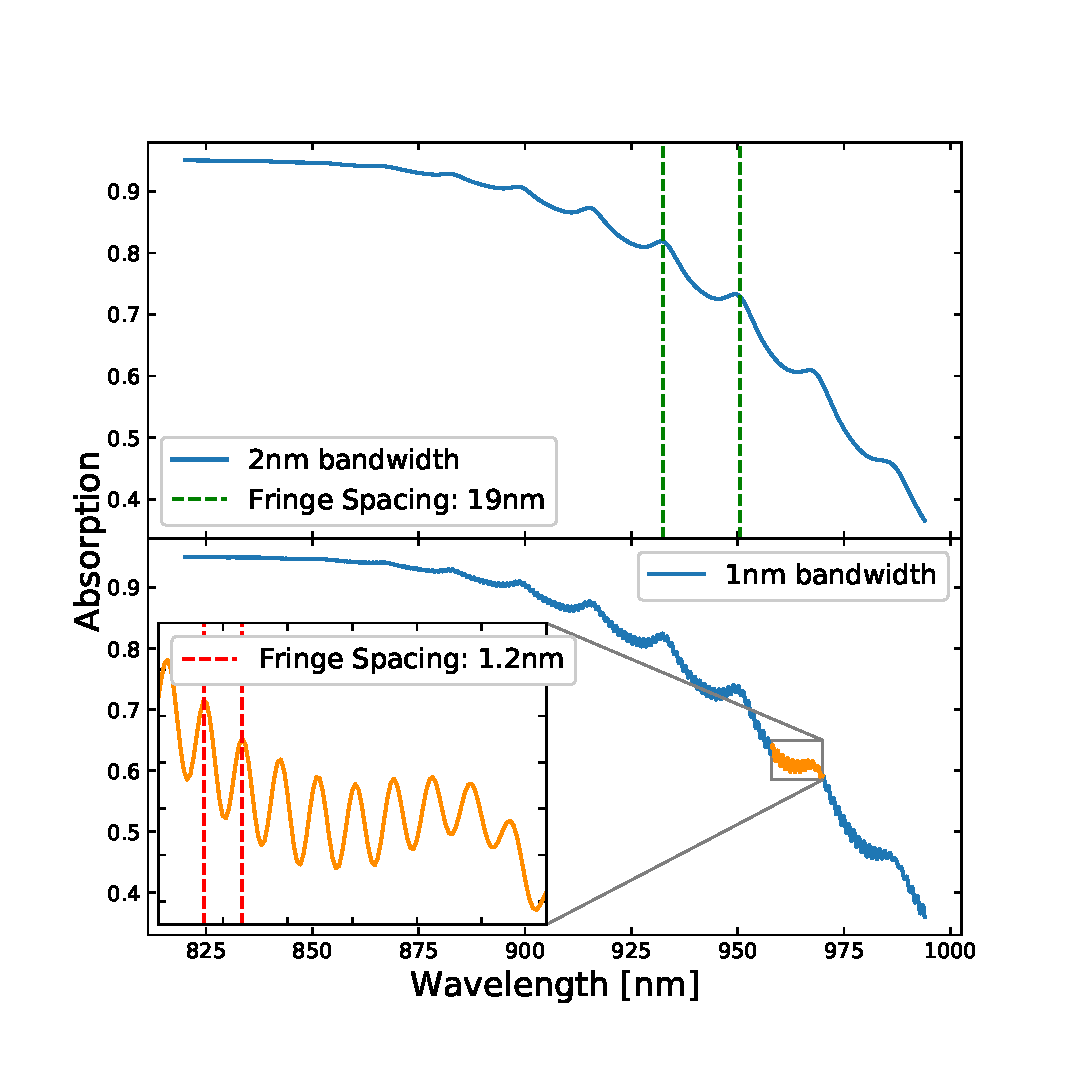
\includegraphics[scale = 0.45]{bandwidth_verify.eps}
\caption{Absorption power versus wavelength of e2v CCD based on different illumination bandwidths. {\it Upper panel:} Calculation based on $2nm$ bandwidth ($d_{epoxy}=14um$ ). Spacing between {\it green dashed lines:} $19nm$ fringe spacing for first fringing pattern related to Epoxy layer. {\it Lower panel:} Calculation results based on $1nm$ bandwidth. Spacing between {\it red dashed lines:} $1.2nm$ fringe spacing for second fringing pattern related to the Si detection layer.}
\label{fig:bandwidth_sim}
\end{figure}
%%%%%%%

%%%%%% Plot: e2v CCD-321 example
\begin{figure}[t]
\centering
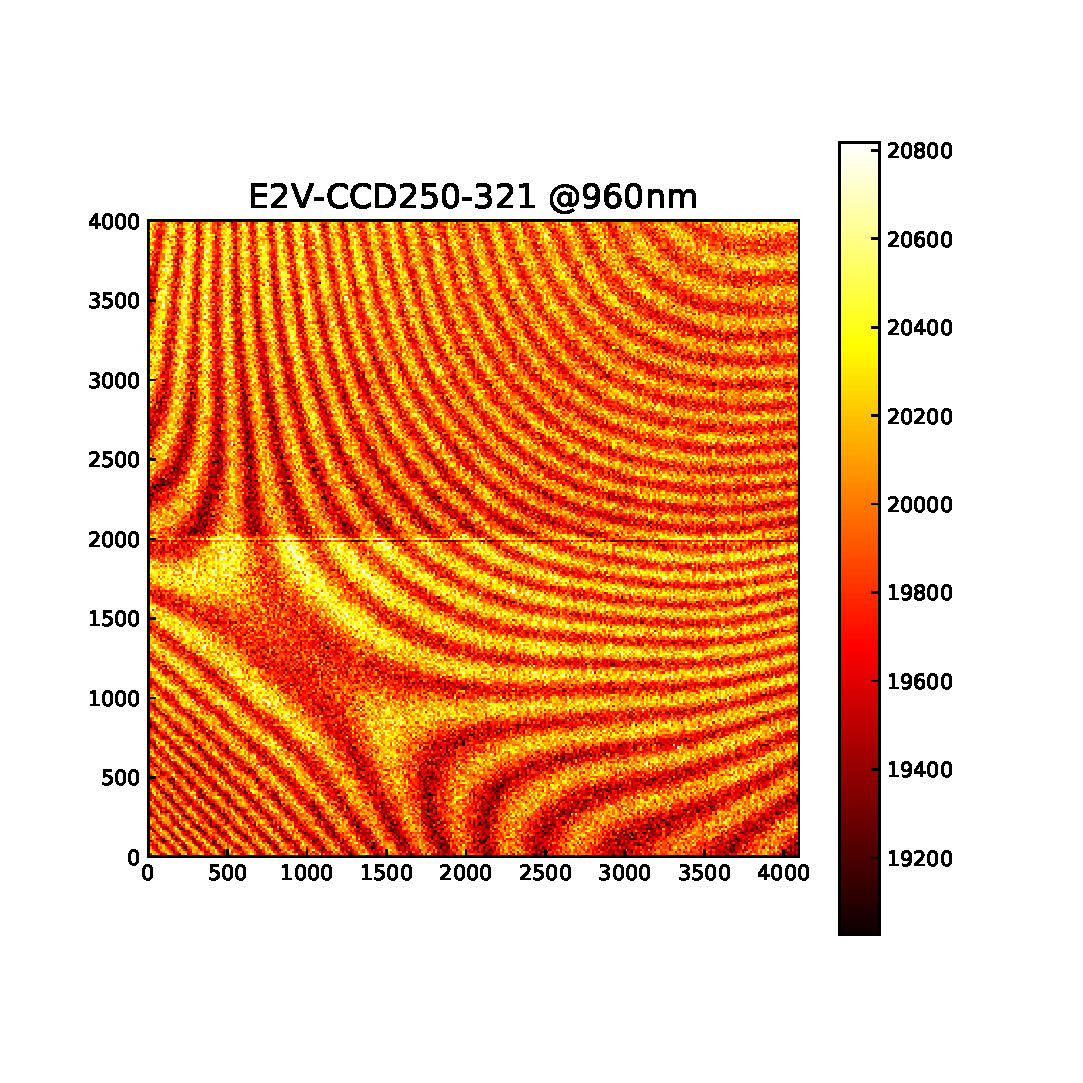
\includegraphics[scale = 0.45]{E2V-321-960nm.eps}
\caption{SLAC-TS8 e2v-321 flat field at $960nm$. The color bar shows the number of electrons per pixel. Only fringing related to the epoxy layer is present, since the fringing caused by the non-uniformity of silicon layer is averaged out by the large bandpass ($2\ nm$) of the monochromator light.}
\label{fig:e2v_example}
\end{figure}
%%%%%%%
This argument is also supported by simulation. Based on the stack model shown in Table \ref{tbl:e2v Structure} with a constant epoxy thickness of $14\mu m$, two sets of simulations with different assumptions for illumination bandwidths, $1nm$ and $2nm$, are generated. A Gaussian distribution is assumed for the monochromatic light profile in which the illumination bandwidth is treated as the Full Width at Half Maximum (FWHM) of the Gaussian. The two panels in Figure~\ref{fig:bandwidth_sim} show absorption power for the stack as a function of wavelength for the two bandwidths respectively. The upper panel shows the calculation results for $2nm$ bandwidth and the calculation for $1nm$ bandwidth is presented in the lower panel. With a 2nm illumination bandwidth, only one fringing pattern with $19nm$ spacing between fringes is observed in the simulation results. Using Eq \ref{eq:Fringe spacing}, it can be easily verified that this spacing corresponds to fringing caused by the $14um$ Epoxy layer with $n_{epoxy} = 1.6$ around $960nm$. With $1nm$ bandwidth, a second fringing pattern with much smaller amplitude appears, as shown in the inset figure in the lower panel. At around $960nm$, the second set of fringes have a spacing about $1.2nm$, coming from the $100um$ Silicon detection layer with monochromatic light of normal incidence.

Before being assembled into the focal plane, CCDs on each LSST science raft are sent to SLAC National Accelerator Laboratory for comprehensive tests and integration \citep{Bond18,Ivezi19}. The data analyzed in this paper comes from SLAC Test Stand 8 (SLAC-TS8). The monochromatic light used to obtain flat field data is generated from a $4"$ integrating sphere which is set $1$ meter away from the CCD. Thus, a collimated beam of light falls at normal incidence is a good approximation, which is the assumption that all the calculations in this section are based on. Figure~\ref{fig:e2v_example} shows an example of the fringing pattern observed in one particular e2v CCD taken under monochromatic light of $2\ nm$ bandpass in SLAC-TS8. It is noticeable that only one fringing pattern is observed in this e2v ccd. this implies that the observed fringing should corresponds to the thickness variation in the epoxy layer since any fringing related to silicon detection layer will be smeared out by the large aperture of the illumination setup.

\textbf{Another test stand with setup identical to SLAC-TS8 was built at Brookhaven Nation Labotory (BNL-TS8) to test LSST CCD sensors as well. BNL-TS8 has a narrower monochromator bandpass of about $1\ nm$. And data taken for e2v sensors in BNL-TS8 indeed shows a second set of fringing pattern, which should be related to the $100\mu m$ silicon based on the conclusions draw from simulation. However, the simulation result implies that the amplitude of the fringes from the epoxy layer is greater than that from the silicon layer.  Additionally, when simulating realistic fringing in telescope image, the simple assumption of normal incident light for lab illumination setup will be replaced with telescope optics, which tends to average out the fringing pattern and further decreases the observed amplitude. See section~\ref{sec: ITL sensor} and section~\ref{sec:LSST optic} for more discussions.} 


%%%%%%%%%%%%%%%%%%%%%%%%%%%%%%%%%%%%%%%%%%%%%%%%%%%%%%%%%%%%%%%%%%%%%%
\subsection{ITL STA3800C CCD} \label{sec: ITL sensor}
\textbf{Fringes are not observed in ITL sensors at SLAC-TS8. This is because ITL sensor has an additional Litho-black coating applied to it. This highly-absorbent black coating will absorb light pass through the epoxy layer and greatly reduce the amount of reflected light from the epoxy~\citep{Connor22}. With illumination light coming from a the monochromator with smaller bandpass compared to SLAC-TS8, fringing is observed in ITL sensors at BNL-TS8. However, \citet{Craig20} have shown that using a $f/1.2$ beam, which is close to the overall focal ratio of LSST telescope ($f/1.23$) \citep{Ivezi19}, fringing is not observed in ITL sensors even with 1nm monochromator bandpass. This supports the argument we made in the end of section~\ref{sec:sensor structure}. Therefore, we conclude that fringing caused by the thickness variation of $100\ \mu m$ silicon layer will be trivial for LSST. And this study focuses on the fringing pattern related to the epoxy layer in e2v sensors.}

%%%%%%%%%%%%%%%%%%%%%%%%%%%%%%%%%%%%%%%%%%%%%%%%%%%%%%%%%%%%%%%%%%%%%%
\section{Fitting thickness of Epoxy layer} \label{sec:Frining_fitting}

%%%%%%%%%%%%%%%%%%%%%%%%%%%%%
\subsection{SLAC Test Stand Flat Fields Data} \label{subsec:SLAC-TS8}

To simulate the observed fringing pattern from the fringing model, the thickness of epoxy layer ($d_{epoxy}$) must be derived at each pixel across the CCD. This is achieved by fitting for $d_{epoxy}$ based on the observed fringing amplitude as a function of wavelength for every pixel of a CCD. Thus, the number of points that are available for fitting is crucial for constraining the thickness of the epoxy layer.
A series of flat fields at different wavelength were obtained for e2v CCD sensors with monochromatic light illumination in SLAC-TS8. The closest wavelength spacing between each successive flat field data available in SLAC-TS8 is $10nm$ for nine e2v sensors in one RTM. 
% (\textbf{e2v-CCD250-319; e2v-CCD250-321; e2v-CCD250-350; e2v-CCD250-357; e2v-CCD250-359; e2v-CCD250-361; e2v-CCD250-363; e2v-CCD250-364; e2v-CCD250-365}) in Raft Tower Module 20 (RTM-020). The data is available in LSST-CAMERA-PORTAL\footnote{\url{https://lsst-camera.slac.stanford.edu}} under run number 10661. 
In the following sections, we describe the method used to derive the epoxy thickness map for each of the nine CCDs.

%%%%%%%%%%%%%%%%%%%%%%%%%%%%%
\subsection{Data Reduction} \label{subsec: data reduction}
The flat field data are preprocessed using LSST Data Management software \citep{Juri17,Axelrod10}. This includes overscan correction that removes the average signal introduced by reading a CCD, and bias subtraction which helps to de-bias a CCD image by subtracting the pixel-to-pixel structure in the the read noise from the raw image. To further reduce the noise level of the preprocessed flat field images, a Gaussian filter with a kernel size of $16$ by $16$ pixels is applied to the overscan corrected image. 

%%%%%% Plot: Si absorption length
\begin{figure}[tb]
\centering
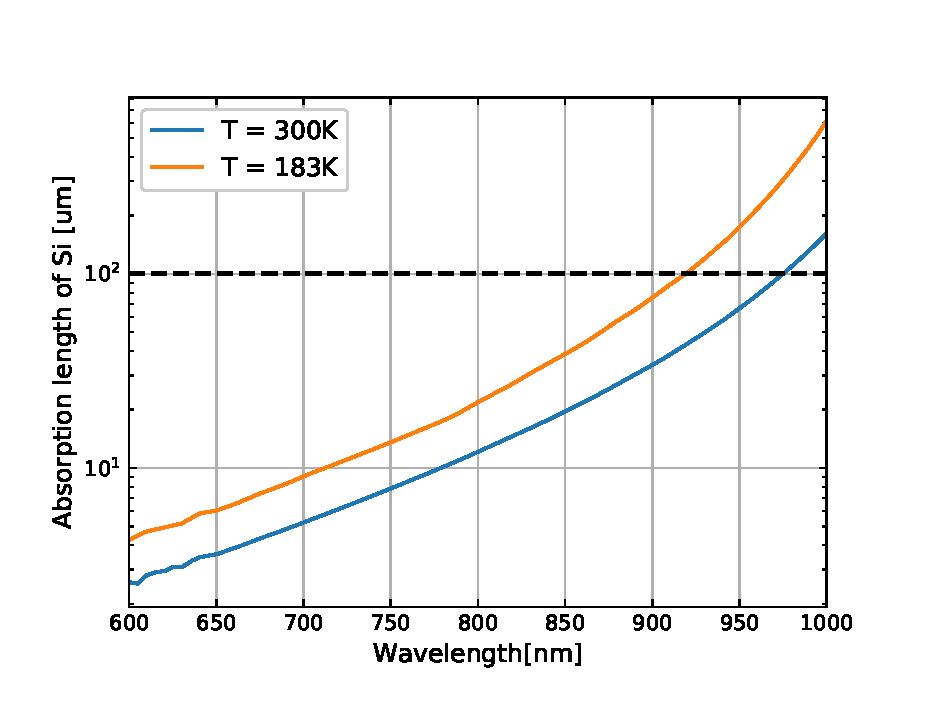
\includegraphics[scale = 0.45]{Si_Absorption_length.eps}
\caption{Depth in Silicon where $99\%$ of incident light is absorbed as a function of wavelength. {\it Blue Solid line:} Room temperature (300K).{\it Orange solid lines:} Temperature = 183K.{\it Dashed black line:} LSST CCD Silicon thickness.The refractive index of Si and temperature coefficients are adopted from \citet{Green08}.} 
\label{fig:Si_ab_length}
\end{figure}
%%%%%%%
SLAC-TS data are taken at temperature of $-90 \degree C$. Figure~\ref{fig:Si_ab_length} shows the absorption depth of silicon, at which $99\%$ of the incident light is expected to be absorbed, as a function of wavelength under two different temperatures. For CCDs with an $100um$ thick silicon operating under $-90 \degree C$, the silicon will become transparent to light at around $900um$. At this point, light will reach the epoxy layer below the $100um$ silicon and some will be reflected back to interfere with incident light in previous layers. Thus, fringes are expected to become prominent in e2v CCDs when the wavelength exceeds $900um$. Based on this conclusion and combined with visual inspection on the test data, fringe flat field data ranging from 880nm to 990nm in steps of 10nm is chosen for fitting the fringing amplitude to derive the value of epoxy layer thickness. The fringing amplitude at an individual pixel is defined as the number of electron counts per pixel over the overall mean number of counts in the image with unity subtracted:

\begin{equation}
    \mbox{Fringe\ Amp.} = \frac{\mbox{Counts}}{\mbox{Overall\ Mean}}- 1
\end{equation}
%%%%%% Plot: Pixle fitting example
\begin{figure}[tb]
\centering
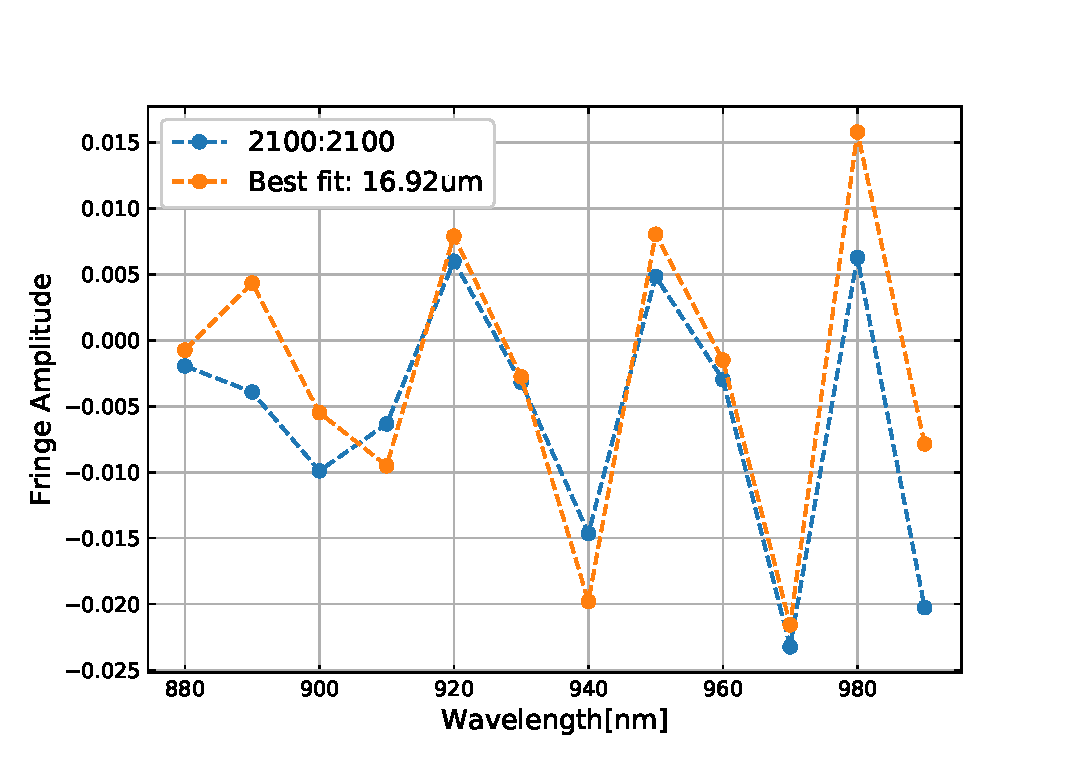
\includegraphics[scale = 0.45]{fit_example.eps}
\caption{Fringing amplitude versus wavelength at the center of e2v-CCD250-321 (pixel 2100,2100) and the best fit fringing model. {\it Red dots:} Fringing amplitude at sampled wavelength at pixel (2100,2100). {\it Blue dashed line:} best fit fringing model for this pixel.} 
\label{fig:Fitting_exmaple}
\end{figure}
%%%%%%%

%%%%%% Plot: e2v-CCD-321 MAP and Simulated Results
\begin{figure*}[hbt]
\centering
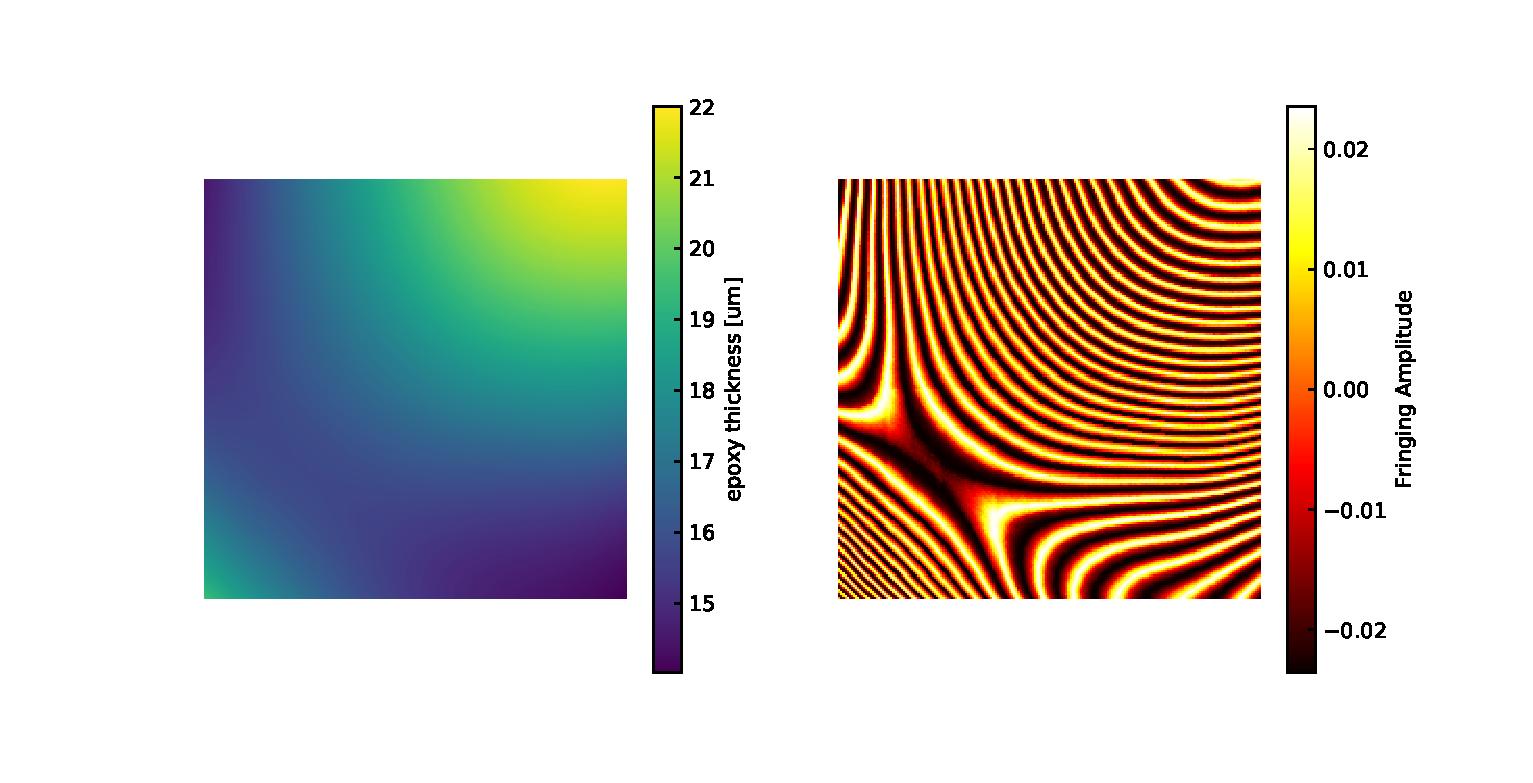
\includegraphics[scale = 0.6]{e2v-321-map_sim.eps}
\caption{{\it Left panel:} Derived epoxy thickness map (4k x 4k pixels) of e2v-CCD250-321.Color bar shows the range of the value of thickness. {\it Right panel:} Simulated fringing pattern based on the derived epoxy thickness map for e2v-CCD250-321. A $2nm$ illumination bandwidth is assumed in simulation. Color bar shows the simulated fringing amplitude.}
\label{fig:321-map-simulation}
\end{figure*}
%%%%%%%
%%%%%%%%%%%%%%%%%%%%%%%%%%%%%
\subsection{Pixel by Pixel Fitting Algorithm}
To get the thickness variation map of the epoxy layer, we adopt the fitting method described in \citet{Malumuth03}.Since only the variation of $d_{epoxy}$ determines the frequency of fringes, the thickness of all the other layers are assumed to be known and the boundary between each layer is assumed to be planar for simplicity (Table \ref{tbl:e2v Structure}). All the calculations are based on the assumption of colliminated beam and $2nm$ illumination bandwidth.
The algorithm contains the following steps: \\ \\
\textbf{Step 1:} An arbitrary pixel (we pick pixel X = 2100, Y = 2100 in the case of e2v-CCD250-321) is chosen as the starting pixel, \textbf{since the final fitting result is insensitive to the location of this starting point.} Then simulated fringing amplitude from $880nm$ to $990nm$ is calculated for a range of epoxy thickness $d_{epoxy}$ ranges from $5um$ to $30um$. \textbf{The value of $d_{epoxy}$ that minimizes the reduced $\chi^2$ of the fit to the observed fringing amplitude is chosen as the best fit ($d_0$) for this starting pixel. The reduced $\chi^2$ is defined as ${\chi^2}$/${(n_d-n_p)}$, with $n_d$ and $n_p$ being the number of data points and number of fitting parameters respectively.} Figure~\ref{fig:Fitting_exmaple} presents the fitting results for this pixel.\\
\textbf{Step 2:} \textbf{We then move to the next pixel in the same column (X = 2100, Y = 2101). Using the derived thickness value of the initial pixel, $d_0$, as a reference point, we calculate the fringing amplitudes for a set of $d_{epoxy}$ values within the range of one order of fringe, $30\ nm$, centered on that value ($d_0\pm 15\ nm$). The order of fringes can be related to varying thickness of epoxy layer ($\Delta d$) via \citep{James87}:
\begin{equation*}
    \Delta d = \frac{\delta \lambda \cos{\theta}}{4\pi n_{epoxy}}
\end{equation*}
In the case of normal incidence, one order of fringe ($\delta = 2\pi$) corresponds to approximately $\Delta d_{epoxy} \approx 30\ nm$.
Within this given range, the value of $d_{epoxy}$ minimizing the reduced $\chi^2$ of the fit is assumed to be the thickness of this pixel. And this value will be updated as the reference point for the next pixel that the algorithm will be working on. Looking for potential best fit values of $d_{epoxy}$ in a limited range in this way helps to ensure the derivation of a smooth thickness variation map of the epoxy layer.}\\
\textbf{Step 3:} Step 2 is repeated until reaching the end of the column (X = 2100, Y = 4000). Then we move down to the next column in that same row (X = 2101, Y = 4000), and work up the row in the same manner as described in previous steps. \\
\textbf{Step 4:} The above steps are repeated until reaching the end (X = 4000, Y = 4000). Upon this point, we move back to the initial pixel (X = 2100, Y = 2100) and repeat the same process in reverse order until reaching pixel X = 1, Y = 1. 


%%%%%%%%%%%%%%%%%%%%%%%%%%%%%
\subsection{Fitting Results}
Figure~\ref{fig:321-map-simulation} shows the derived epoxy layer thickness map of e2v-CCD250-321 in the left panel. Using the fringing model, we successfully reproduced the observed fringing pattern, which is shown in the right panel in Figure \ref{fig:321-map-simulation}, based on this derived height variation map. The simulation result is based on the assumption of a $2nm$ illumination bandwidth.
%%%%%% Plot: e2v-CCD-321 MAP and Simulated Results
\begin{figure}[hbt]
\centering
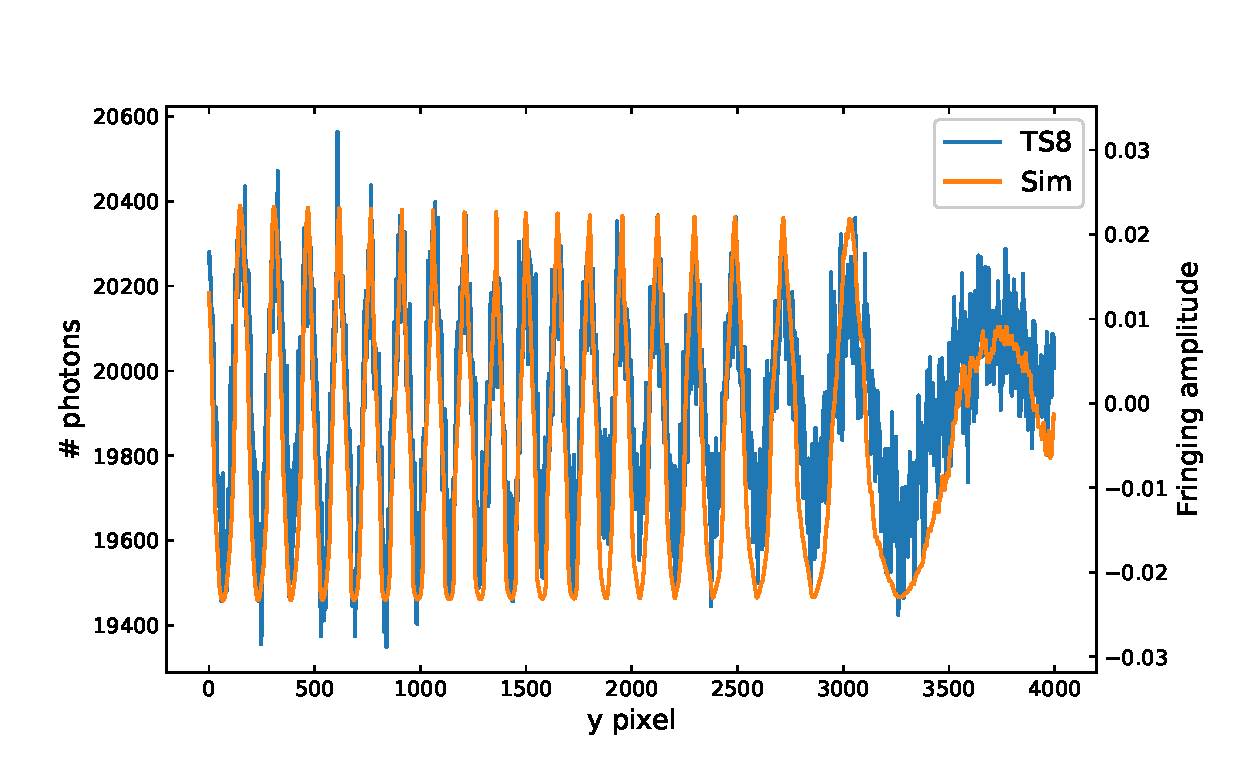
\includegraphics[scale = 0.4]{E2V-321-detail-compare.eps}
\caption{Comparison between data and simulation for e2v-CCD250-321 column 3000. {\it Blue solid line:} Smoothed SLAC-TS8 flat field data. {\it Orange dashed line:} simulated results under the assumption of 2nm illumination bandwidth.}
\label{fig:321-detail-compare}
\end{figure}
%%%%%%%
Figure~\ref{fig:321-detail-compare} shows the comparison between Gaussian-smoothed real data and simulation results for a specific row of the sensor. It is clear that the phases and amplitudes are matched for most parts between simulation and real data.


\begin{figure*}[tbh]
\centering
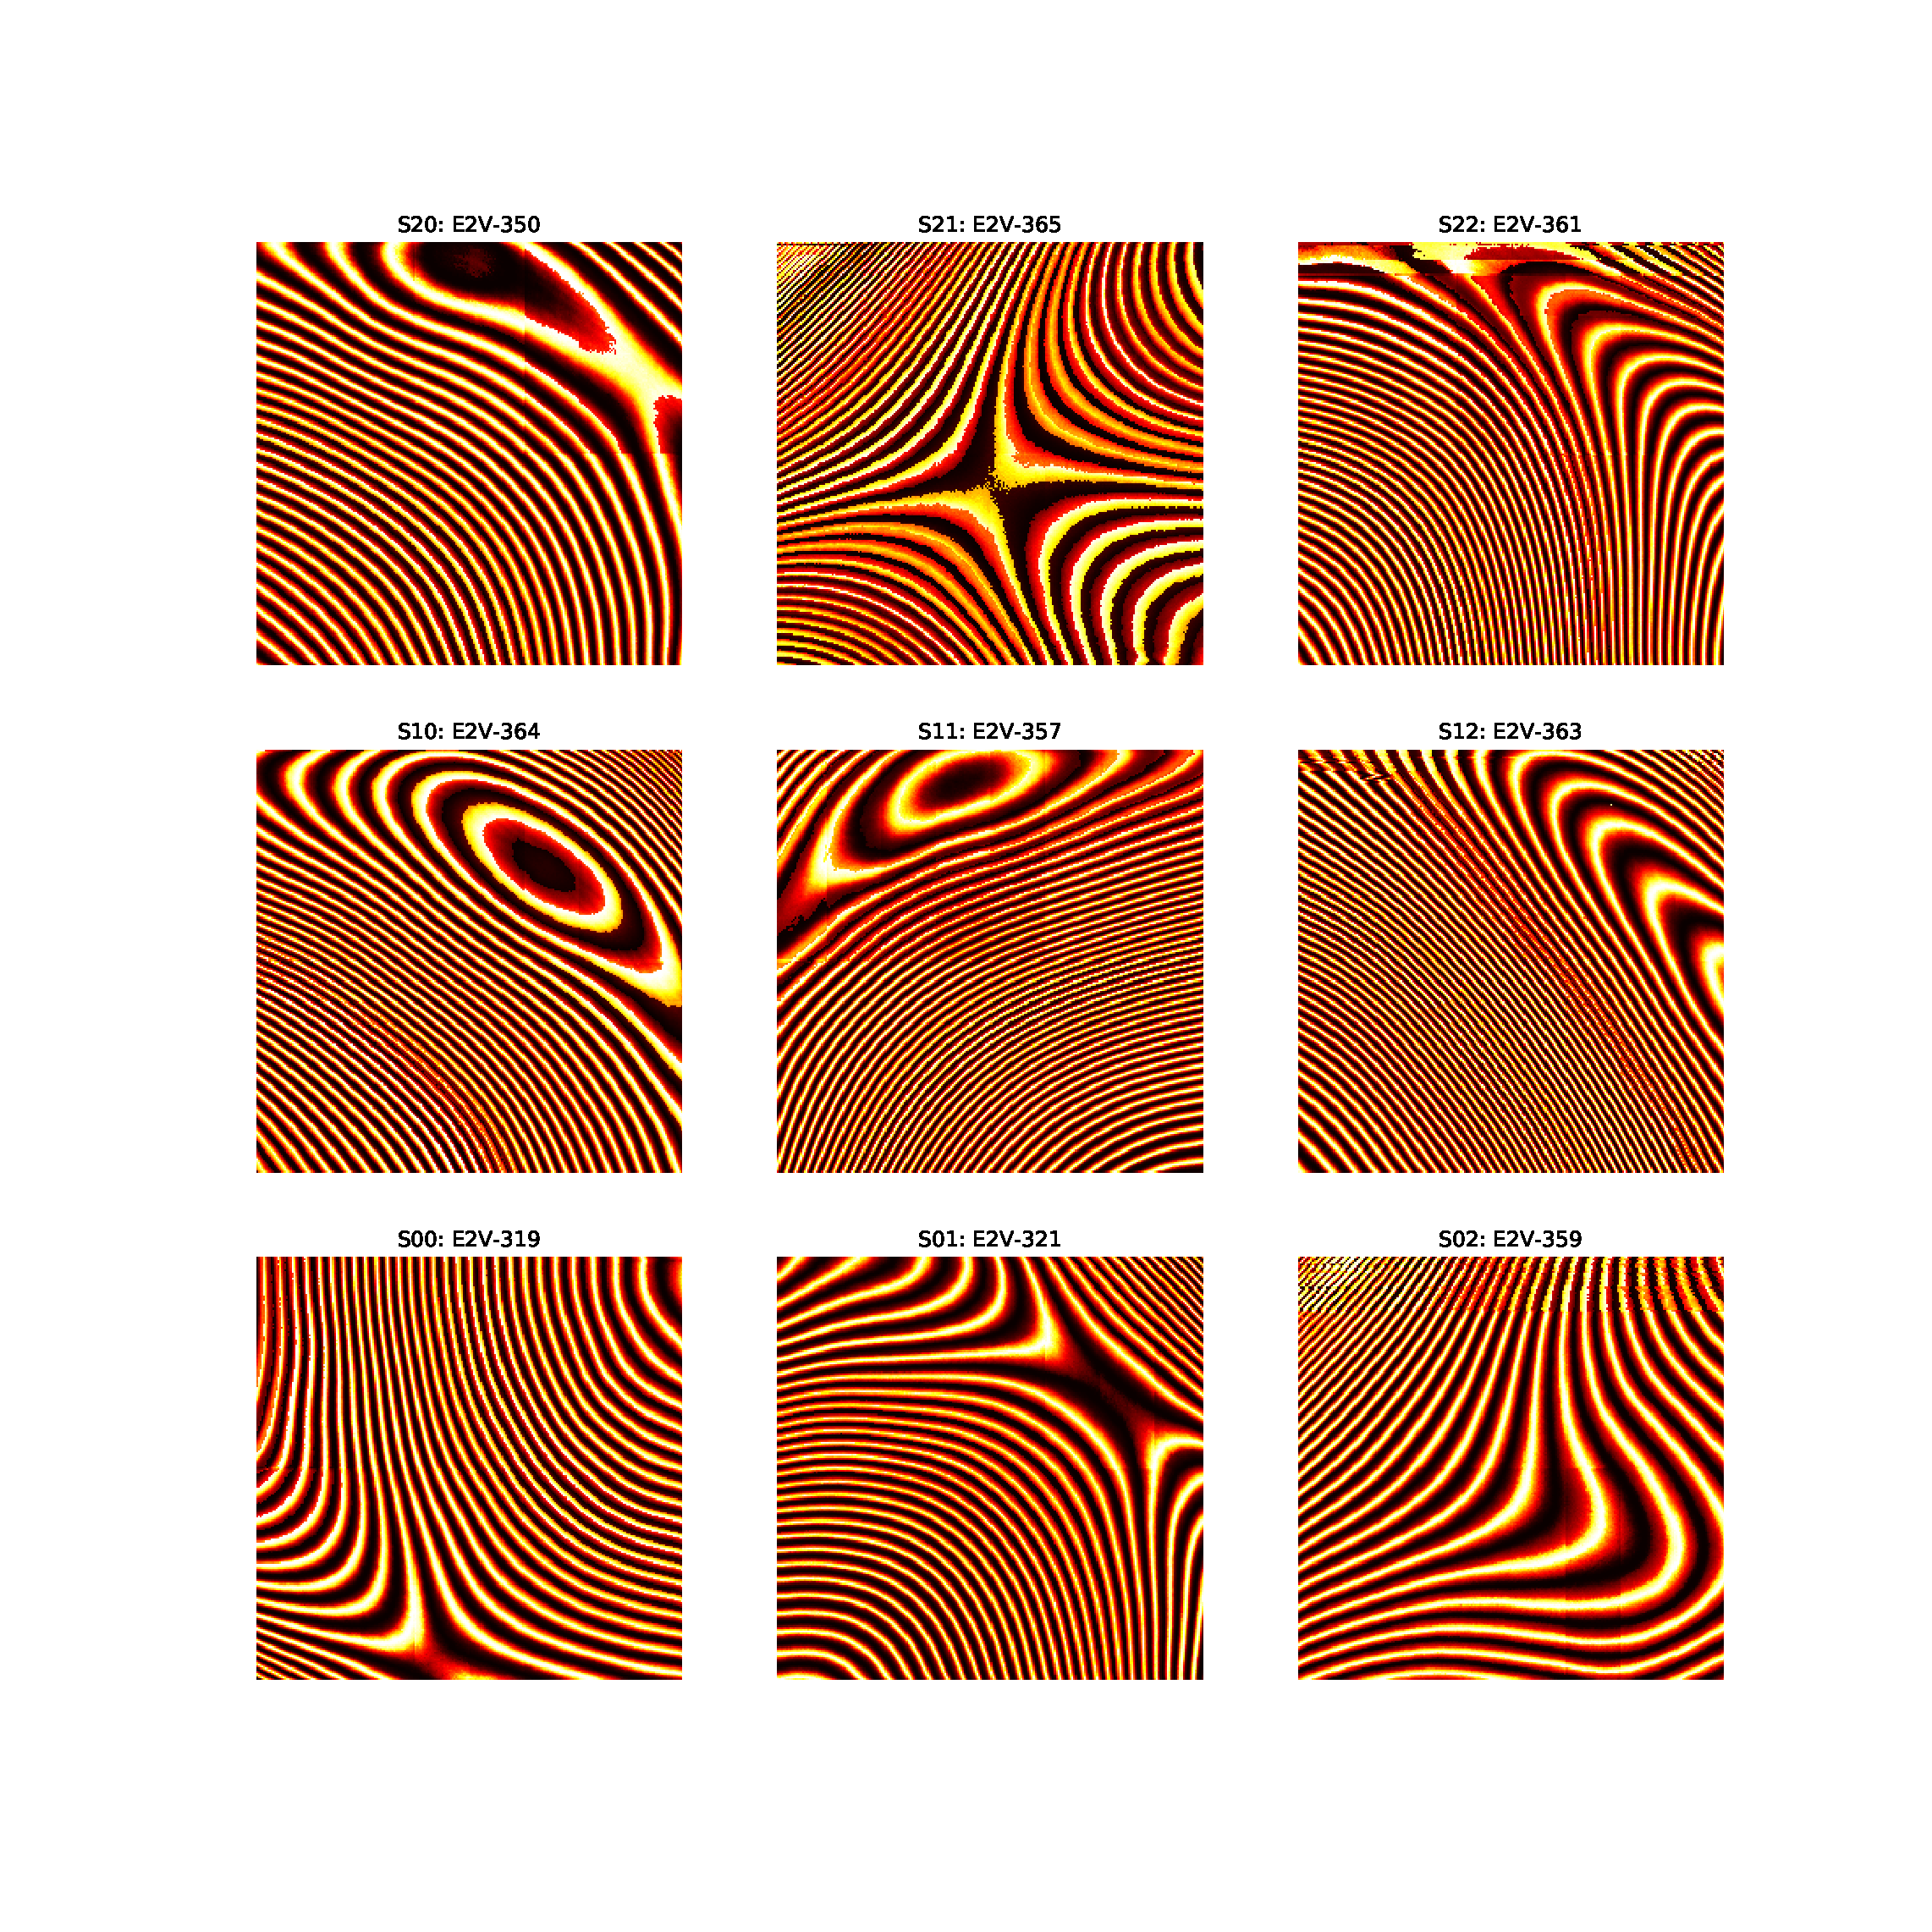
\includegraphics[scale = 0.45]{RTM-020-Sim.eps}
\caption{Simulated fringing pattern (with illumination bandwidth being a delta function at 960nm) based on derived epoxy thickness map for nine e2v CCDs in RTM-020}
\label{fig:RTM-020-SIMS}
\end{figure*}

Using this method, we generate the fringing patterns observed in the other 8 sensors in the same RTM from simulation. Figure~\ref{fig:RTM-020-SIMS} shows the simulated fringing patterns for all these nine CCDs. Most of the fringing patterns have been successfully recovered.

%%%%%%%%%%%%%%%%%%%%%%%%%%%%%%%%%%%%%%%%%%%%%%%%%%
\section{Recipes for Realistic fringing simulation in sky background image} \label{sec:recipes for real image}
With knowledge of the composition of sensor structure and height variations in the epoxy, we can further use the fringing model to predict the expected level of fringing in LSST images. In this section, we discuss all the ingredients needed to simulate fringing in real sky images captured by a telescope in general.  

\subsection{Hydroxyl Radical (OH) emission lines}\label{sec: OH line + y filter}
 The night sky spectrum is dominated by the emission lines produced by the rotational and vibrational transitions of hydeoxyl (OH) radicals being excited by Sun light, especially in the near-infrared wavelength. Each vibrational transition produces a band in the observed spectrum and the transition between rotational levels asscioated with the two vibrational levels give rise to the fine structure of the band. The vibration-rotation spectrum of the hydroxyl radical were first observed by \citet{Meinel50a,Meinel50b}.
%%%%%%%%%%%%%%%%%%%
\begin{figure*}[htb]
\epsscale{0.85}
\centering
\plotone{OH_spec2.eps}
\caption{\textbf{Top panel:} {\it Light blue line:} OH emission line from the Prime Focus Spectrograph (PFS) of the Subaru telescope~\citep{Tamura16}. {\it Red dahsed line:} LSST y filter throughput with LSST sensor QE divided out. {\it Black dahsed line:} HSC y filter throughput with HSC sensor QE divided out. \textbf{Bottom panel:} {\it Blue line:} Normalized output of OH line intensity weighted by LSST y filter throughput.}
\label{fig:OH_spec}
\end{figure*}
%%%%%%%%%%%%%%%%%%%
These narrow emission lines are the main sources that give rise to fringing in the observed images, and are expected to dominate the upper atmosphere spectra. The intensity of vibrational bands and the population of rotational levels within each band can be well described by Boltzmann distributions specified by vibrational temperatures, $T_{vib}$ and rotational temperatures, $T_{rot}$. The typical values of $T_{vib}$ and $T_{rot}$ are about $10000K$ and $200K$ respectively~\citep{Rousselot00}, and they are subject to both temporal and spatial variations.  Nevertheless, the relative intensities of rotational transition lines are expected to remain roughly on the same level since $T_{rot}$ varies on a much less than $T_{vib}$~\citep{Noll15,Hart19}.

As discussed in section~\ref{subsec: data reduction}, fringing will become prominent in e2v sensors as the wavelength goes beyond $900nm$. Real images are taken under filters and, the wavelength relevant to fringing falls within the range covered by the LSST y filter. The top panel in Figure~\ref{fig:OH_spec} shows the OH emission spectra taken by the Prime Focus Spectrograph (PFS) \citep{rlh} of the Subaru telescope~\citep{Tamura16}. As confirmed by observations and theoretical calculations in previous studies, there are six transitions between vibrational bands ($7-3$, $8-4$, $3-0$, $9-5$, $4-1$, $5-2$) within the range covered by LSST y filter~\citep{Noll15,Osterbrock96,Osterbrock97,Rousselot00}. The color coding of the lines in Figure~\ref{fig:OH_spec} represents the vibrational group lines belongs to. 

\begin{figure}[htb]
\epsscale{1.1}
\centering
\plotone{det_response.eps}
\caption{LSST generic detector response curve ({\it Blue dashed line}) and the detector response curve calculated from the fringe model used in this paper ({\it Yellow solid line}).}
\label{fig:det_response}
\end{figure}


In simulating fringing caused by OH lines, the contribution of each individual line in the spectra is obtained via weighting the intensity of each line with the throughput of LSST y band shown in Figure~\ref{fig:OH_spec}. The filter throughput curve combines LSST baseline curve of filter, optics, mirrors, atmosphere and detector response together~\citep{Ivezi19}. It is noteworthy that since detector response (QE $+$ AR coating) is inherited in the fringing model, this response curve is divided out from the total throughput when weighting the OH lines. Figure~\ref{fig:det_response} shows the generic LSST detector response curve used to calculate filter throughput and the one derived from the fringe model used in this study. The bottom panel in Figure~\ref{fig:OH_spec} shows the normalized line weight. Due to the low throughput of LSST y filter at around $900nm$ , the contributions to fringing from lines in vibrational groups $7-3$ is minimal compared to other groups. The final simulation result, $F_{total}$, is obtained by stacking the simulation for each individual line, $F_{line}$, with proper weight, $w_{line}$:

\begin{equation*}
    F_{total} = \sum_{line}w_{line}\cdot F_{line}
\end{equation*}

%%%%%%%%%%%%%%%%%%%%%%%%%
\begin{figure}[t]
\centering
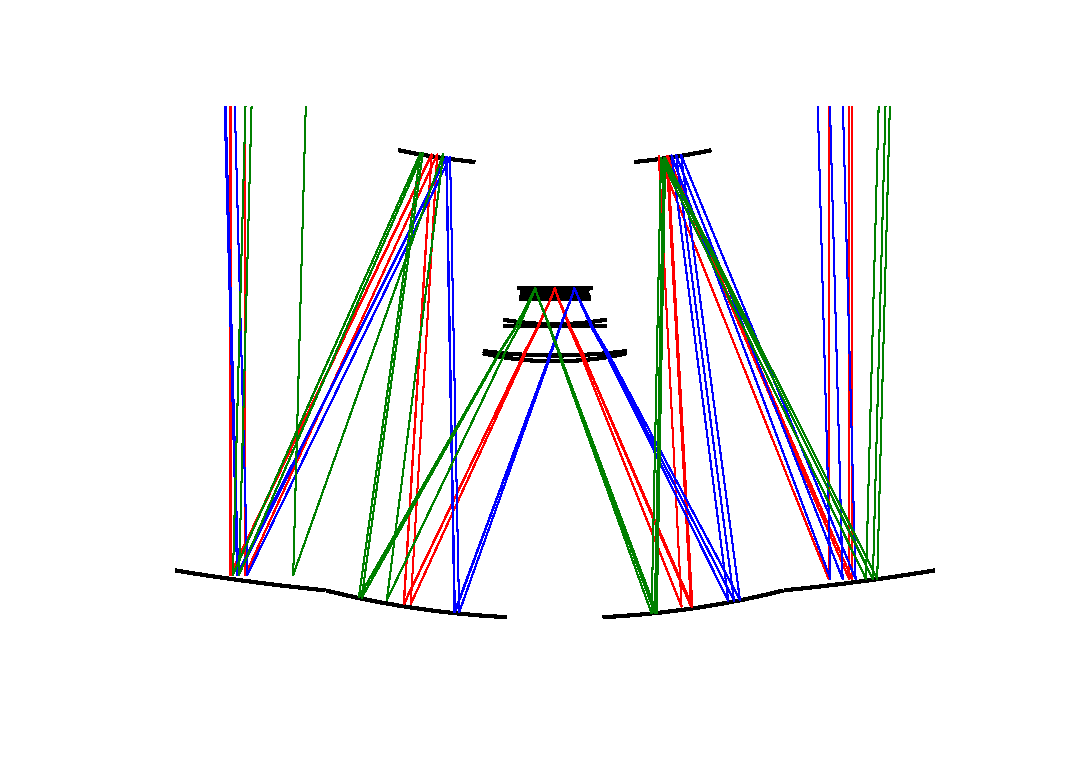
\includegraphics[scale = 0.4]{light_tracing.eps}
\caption{Light path inside the LSST telescope calculated using Batoid.}
\label{fig:batoid-light-tracing}
\end{figure}
%%%%%%%%%%%%%%%%%%%%%%%%%


\subsection{Telescope optics} \label{sec:LSST optic}



An actual instrument, such as telescope, has a finite aperture that makes the incident light come from a range of angles rather than solely at normal incidence. Thus, the previous assumption of collimated beams used in simulating lab results does not hold true anymore. And lights arriving at different angles tend to average out the observed fringing amplitude~\citep{Groom17}. The LSST telescope is a three-mirror telescope. The three aspheric mirrors, an 8.4m primary mirror, a 3.4 m convex secondary mirror, and a 5.0 m tertiary mirror, give an overall focal ratio of $f/1.234$ \citep{Bond18,Ivezi19,Olivier08}. To accurately count the range of light incident angle from the $f/1.234$ beam on different positions of the LSST focal plane in fringing simulation, we employ Batoid. Batoid is a C++ based python optical raytracer package that characterizes the optical performance of survey telescopes based on geometric optics developed by \citet{Mayers19}. Figure~\ref{fig:batoid-light-tracing} demonstrates some examples of light paths inside the LSST telescope generated by Batoid. In Batoid, the directions of the incident beams are described by incoming slopes in two directions $\frac{dx}{dz}$ and $\frac{dy}{dz}$. The incident angle $\theta$ on the incidence plane, one of the inputs of the fringing model, can be derived from the two slopes: 

\begin{equation*}
    \theta (\mbox{rad}) = \arctan{\sqrt{\left(\frac{dx}{dz}\right)^2+\left(\frac{dy}{dz}\right)^2}}
\end{equation*}
Figure~\ref{fig:batoid-angle-dist} shows the incident slope distributions of light landing on CCDs in two different locations on the LSST focal plane, one with the sensor located in the center and the other at the edge at the LSST focal plane~\citep{Ivezi19}.

\begin{figure}[t]
\centering
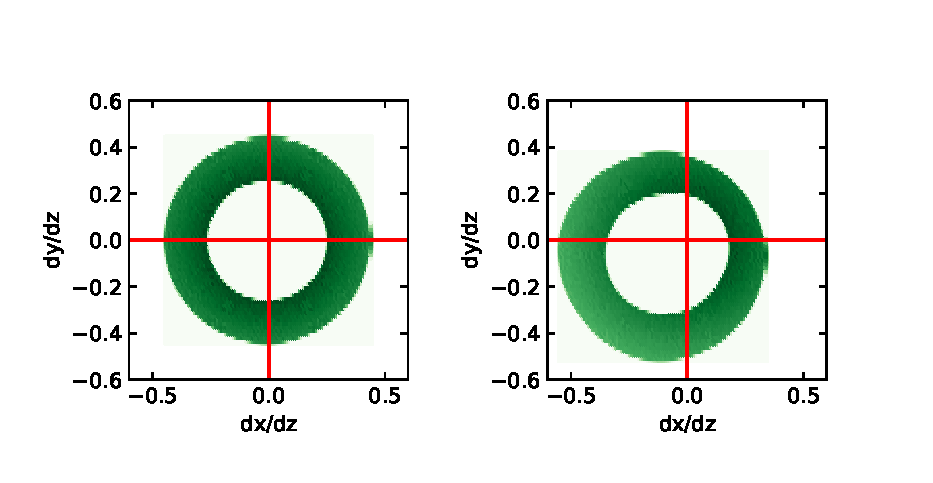
\includegraphics[scale = 0.55]{batoid_angle_dists.eps}
\caption{Incident slope distribution of light beam in two different places of the LSST focal plane. {\it Left panel:} Incident slope distribution of LSST beam landed on the center of the focal plane. {\it Right panel:} Incident slope distribution close to the edge of the focal plane.}
\label{fig:batoid-angle-dist}
\end{figure}

\begin{figure*}[thb]
\epsscale{0.85}
\centering
\plottwo{ab_photon_dist_center.eps}{ab_photon_dist_edge.eps}
\caption{Distribution of travelling distance in Silicon of absorbed photons in two different places of the LSST focal plane. {\it Left plot:} in the center of the focal plane. {\it Right plot:} close to the edge of the focal plane. The color coding in indicates the depth in Silicon a photon has travelled. The lighter the color, the deeper a photon goes into the Silicon before getting absorbed.}
\label{fig:ab_pho_dist}
\end{figure*}


The incident inclination of LSST beam makes it possible for absorbed photons in photo-sensitive region to travel into neighbouring pixels instead of staying in the same pixel where it initially landed on in the case of normal incidence. To check if this may affect the fringing simulation results in a significant way, we did a detailed simulation in which each absorbed photon is tracked to its final location where the electron-photon pair is generated in the photo-sensitive region of CCD. Figure~\ref{fig:ab_pho_dist} presents the distribution of the distances photons have travelled in x and y directions as specified by the two slopes before getting absorbed in Silicon for 1000 photons assumed to be landed at the center of a pixel.  The two cases presented in Figure~\ref{fig:ab_pho_dist} correspond to the angle distributions showed in Figure~\ref{fig:batoid-angle-dist}. The color coding indicates the z direction (depth) that a photon has travelled in Silicon. Lighter color corresponds to deeper distance a photon has travelled in the silicon before getting absorbed. Each pixel in LSST CCD sensor is $10\mu m$ in width and length, and $100\mu m$ in depth~\citep{Ivezi19}. \textbf{Simulation results in Figure~\ref{fig:ab_pho_dist} indicate that even when the light lands the focal plane edge, $98\%$ of the absorbed photons will travel less than the size of one pixel ($10 \mu m$) in both x and y directions.} We consider this effect to be negligible for the purpose of simulating the fringing pattern of 4000 by 4000 pixels images. Thus, to save computational time, an absorbed photon is always assumed to be ended up in the same pixel as the one it initially landed on. Additionally, the distribution of incident slopes of light is assumed to be constant for all pixels of a CCD since this distribution is expected to vary very slowly across the focal plane.



%%%%%%%%%%%%%%%%%%%%%%%%%%%%%%%%%%%%%%



\section{Fringing simulation results} \label{sec:real_sky}
To verify the robustness of the fringing model in simulating real sky images, we first applied it to simulate sky background fringing for MonoCam \citep{Brooks17} and Hyper-Sprime Camera (HSC) \citep{Miyazaki18} before making predictions for LSST. In this section, we first discuss the comparison between simulation results and observation in terms of the optics setup of MonoCam and HSC. Then we use the fringing model to predict the expected level of fringing in LSST images. All simulations in this section follow the methods described in section~\ref{sec:recipes for real image}.

\subsection{Fringing of MonoCam} \label{sec: MonoCam sim}
%%%%%%%%%%%%%%%%%%%%%%%%%%%%%%%%
\begin{figure*}[thb] 

\epsscale{1}
\centering
\plottwo{MonoCam_sims.eps}{MonoCamimage.eps}
\caption{{\it Left plot:} Simulated fringing amplitude for the diagonal pixels of e2v-CCD250-321 based on OH emission lines, MonoCam optics and LSST y filter. {\it Right plot:} 4kx4k simulated MonoCam midnight sky background image with Poisson photon noise and Gaussian read noise added. Color bar represents the number of electron counts per pixel.}
\label{fig:MonoCam_sims}
\end{figure*}
%%%%%%%%%%%%%%%%%%%%%%%%%%%%%%%%

%%%%%%%%%%%%%%%%%%%%%%%%%%%%%%%%%%
\begin{figure*}[bt]
\centering
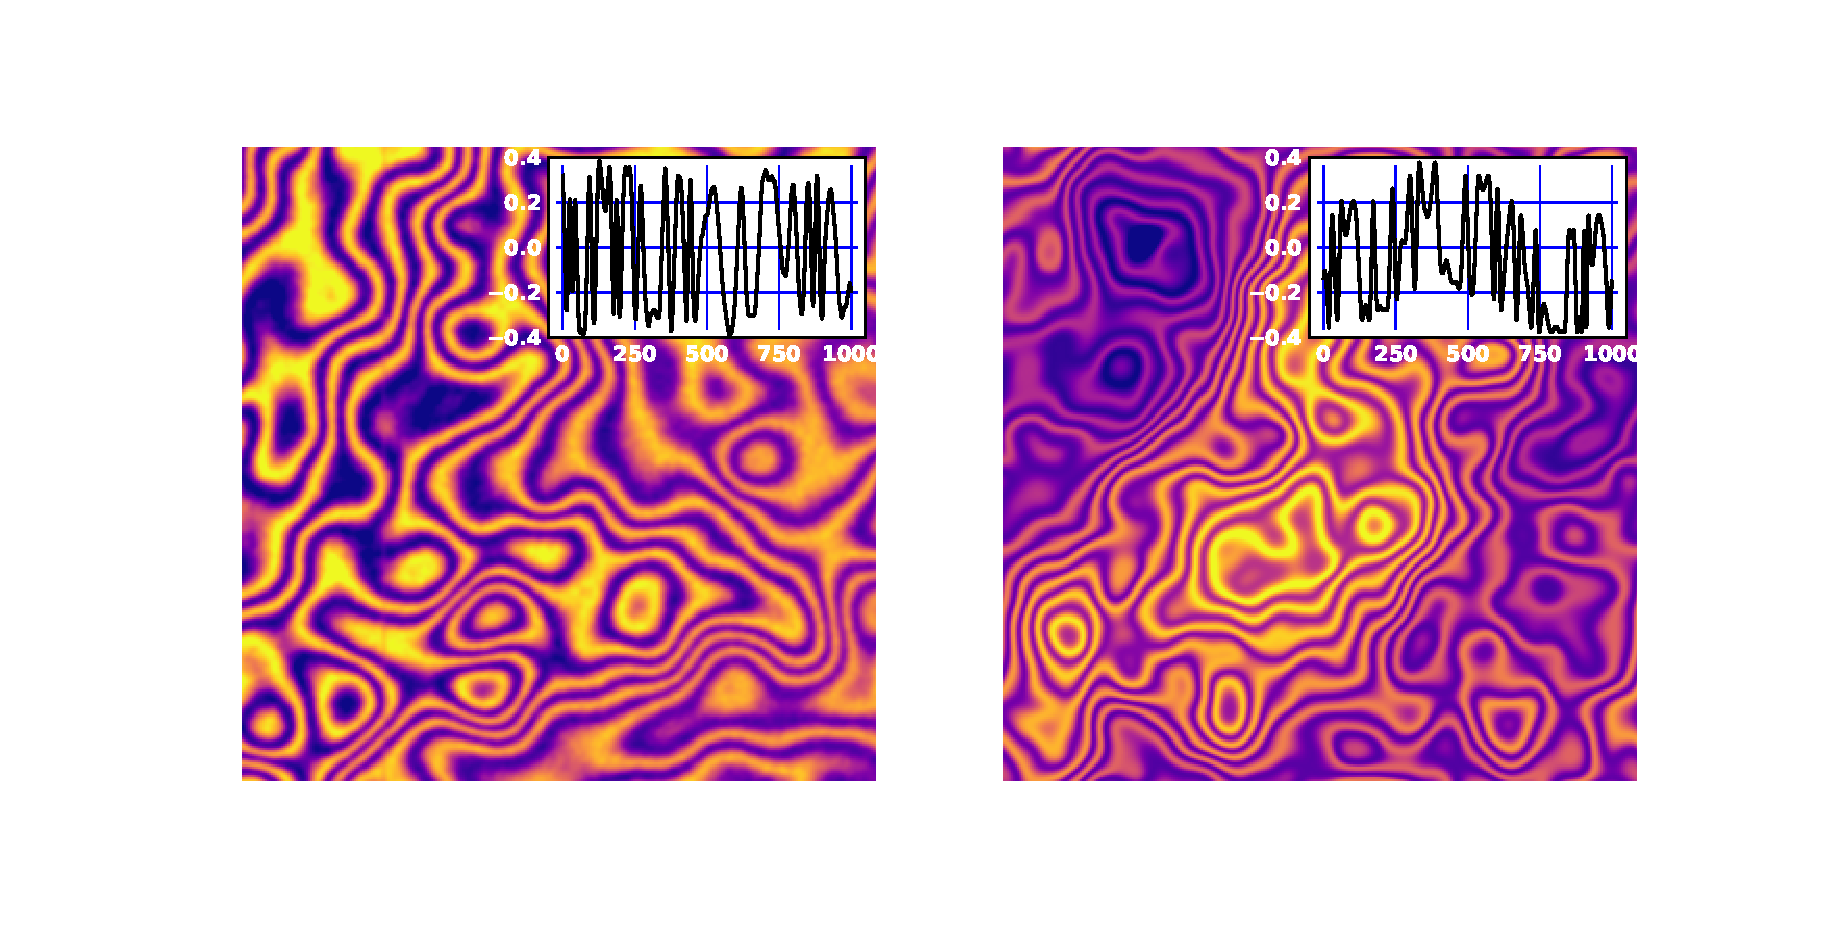
\includegraphics[scale = 0.5]{HSC-data-sim.eps}
\caption{Fringing in HSC CCD. {\it Left panel}: Fringing observed in a 1000 by 1000 pixel region of a single HSC CCD sensor. {\it Right panel}: Simulated HSC fringing pattern based on OH emission lines, HSC optics and HSC y filter throughput. The mini panel in the top right of each figure shows the variation of percentage fringing amplitude along the diagonal pixels.}
\label{fig:HSC_sims}
\end{figure*}
%%%%%%%%%%%%%%%%%%%%%%%%%%%%%%%%%

MonoCam was a camera employing a single LSST prototype e2v-CCD250 sensor, with reported fringing amplitude of around $2\%$. The data where taken with a 1.3m reflector telescope with a overall focal ratio of $f/4.0$ and with LSST y filter under a temperature of $-120\degree C$ \citep{Brooks17}. Since the CCD used in MonoCam came from the same manufacturer as the sensor studied in this paper, the derived epoxy thickness map of e2v-321 is assumed for this prototype sensor for the purpose of fringing simulation. The $f/4.0$ telescope focal ratio infers a light incident range from $0$ deg to $7.1$ deg for MonoCam.

The left panel of Figure~\ref{fig:MonoCam_sims} presents the fringing amplitude of the diagonal pixels of the simulated, noiseless image. The simulation result shows that the MonoCam fringing amplitude is about $1.5\%$, which agrees to the amplitude of the smoothed and noise-reduced midnight fringing pattern given in Figure 9 of \citet{Brooks17}. A full sensor image of the simulated sky background is shown in the right panel of Figure~\ref{fig:MonoCam_sims} based on the $60$ seconds MonoCam exposure time \citep{Brooks17}. Poisson photon noise and Gaussian read noise are added to the simulated full image by using the Galsim module~\citep{Galsim}. It is clear that nontrivial fringing pattern still appears in the image. These results suggest that our fringing model simulation is in well agreement with MonoCam observations.

\subsection{Fringing in HSC CCD sensor}

HSC is an $870$ megapixel prime focus optical imaging camera with a overall focal ratio of $f/2.0$ for the $8.2$ m Subaru telescope. $116$ Fully-depleted  2048 × 4096 pixel CCDs with a thickness of $200\mu$m are employed in the focal plane \citep{Miyazaki18}. The HSC optics offers an opportunity to test the fringing model's response to a fast input beam . From the inspection of real HSC sky images, it is found that fringing of HSC CCD has a sensor dependent amplitude ranging from $0.2\%$ to $0.6\%$. As an example, the left panel of Figure~\ref{fig:HSC_sims} shows the observed fringing pattern in a 1000x1000 pixel region of an HSC CCD. To reduce the noise and make fringes easier to see, the plotted data have been smoothed by a 16x16 pixel gaussian kernel. The mini panel in the top right of the figure shows the fringing amplitude, which is about $0.3-0.4\%$, along the diagonal pixel of the image. Fringes in HSC CCDs are likely to be caused by the non-uniformity in the $200\mu m$ silicon layer. This is because they exhibit similar features as the ones observed in other back-illuminated sensors, such as the HRC CCD and WFC CCD, whose fringes are modelled based on height variation in silicon detection layer, studied by \citet{Walsh03}. 

To simulate HSC sensor fringing, we made the following changes to the sensor model as depicted in Table~\ref{tbl:e2v Structure}. First, the thickness of epoxy is kept constant at $14\mu m$ since HSC CCD fringing is caused by non-uniformity in 200$\mu m$ silicon in stead of epoxy as discussed above. Second, a Guassian Random Field (GRF) is used to model the variation of the detection layer. Since our goal in this section is to verify if the fringing model produce similar level of fringing amplitude as ones inferred from real HSC images, the actual fringing pattern and image size can be arbitrary. Thus, a GRF is a good approximation to the underlying variation of the silicon layer. For this case, we used a GRF, with a size of 1000 by 1000 pixel, that returned \hl{ a overall variation of $1 \mu m$ across the $200\mu m$ silicon.} \textcolor{red}{(needs to be verified)} Batoid is then used to generate the angle distribution of the incident beam in the center of the focal plane based on HSC telescope optics. The OH line intensities are weighted with the throughput curve of HSC y filter was done in Figure~\ref{fig:OH_spec}. Again, the QE curve of the HSC sensor is divided out from the total throughput curve as discussed in section~\ref{sec: OH line + y filter}. In the right panel of Figure~\ref{fig:HSC_sims}, we present the simulated 2D fringing pattern and amplitude across the diagonal pixels of simulated image. It is clear that the predicted  amplitude ($\sim 0.3\%$) is comparable to the observed level in the left panel.

\subsection{Prediction of Fringing in LSST real sky image}
%%%%%%%%%%%%%%%%%%%%%
\begin{figure}[htb]
\centering
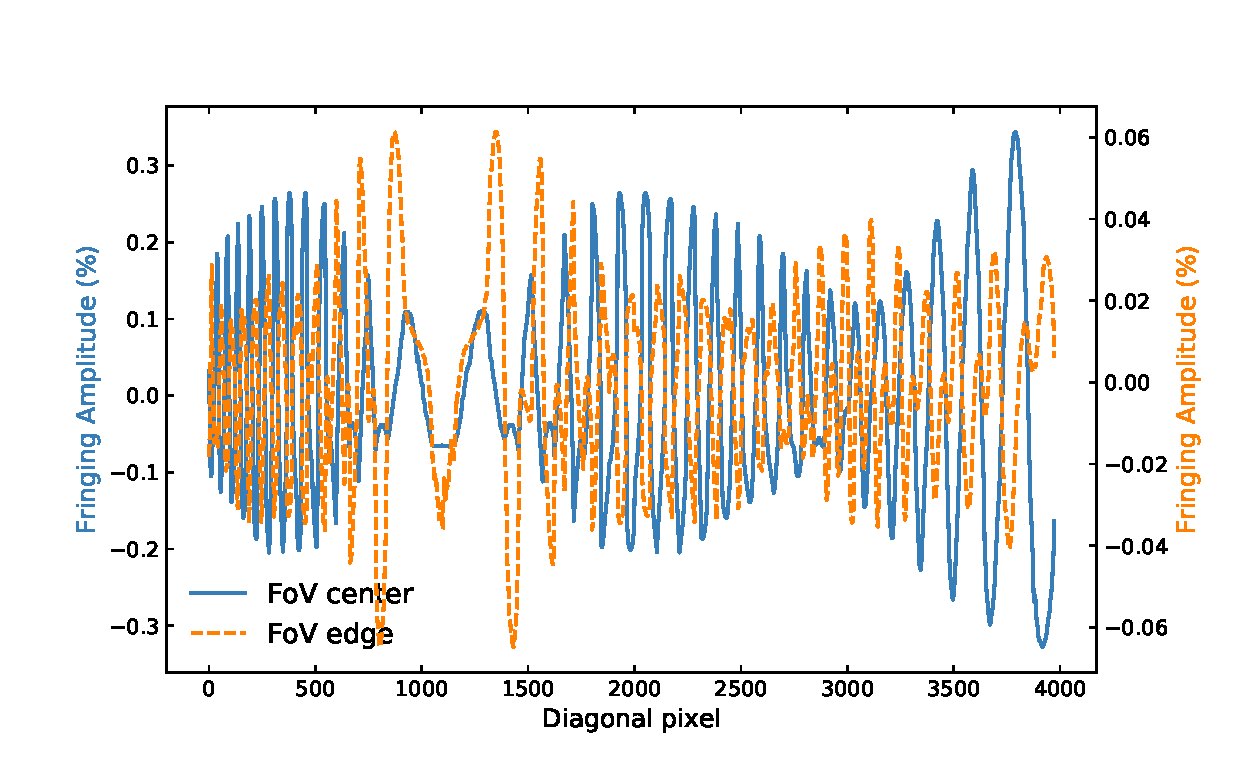
\includegraphics[scale = 0.41]{LSST-fringe-sims.eps}
\caption{Simulated fringing pattern at different locations on the LSST focal plane for diagonal pixels of e2v-CCD250-321 based on LSST optics setup. {\it Blue, solid line:} sensor at the center. {\it Orange, solid line:} sensor being at the edge of the focal plane. The corresponding angle distributions of incident beam for the two cases are given in Figure~\ref{fig:batoid-angle-dist}.}
\label{fig:LSST_sims}
\end{figure}
%%%%%%%%%%%%%%%%%%%%%

%%%%%%%%%%%%%%%%%%%%%
\begin{figure*}[tbh]
\centering
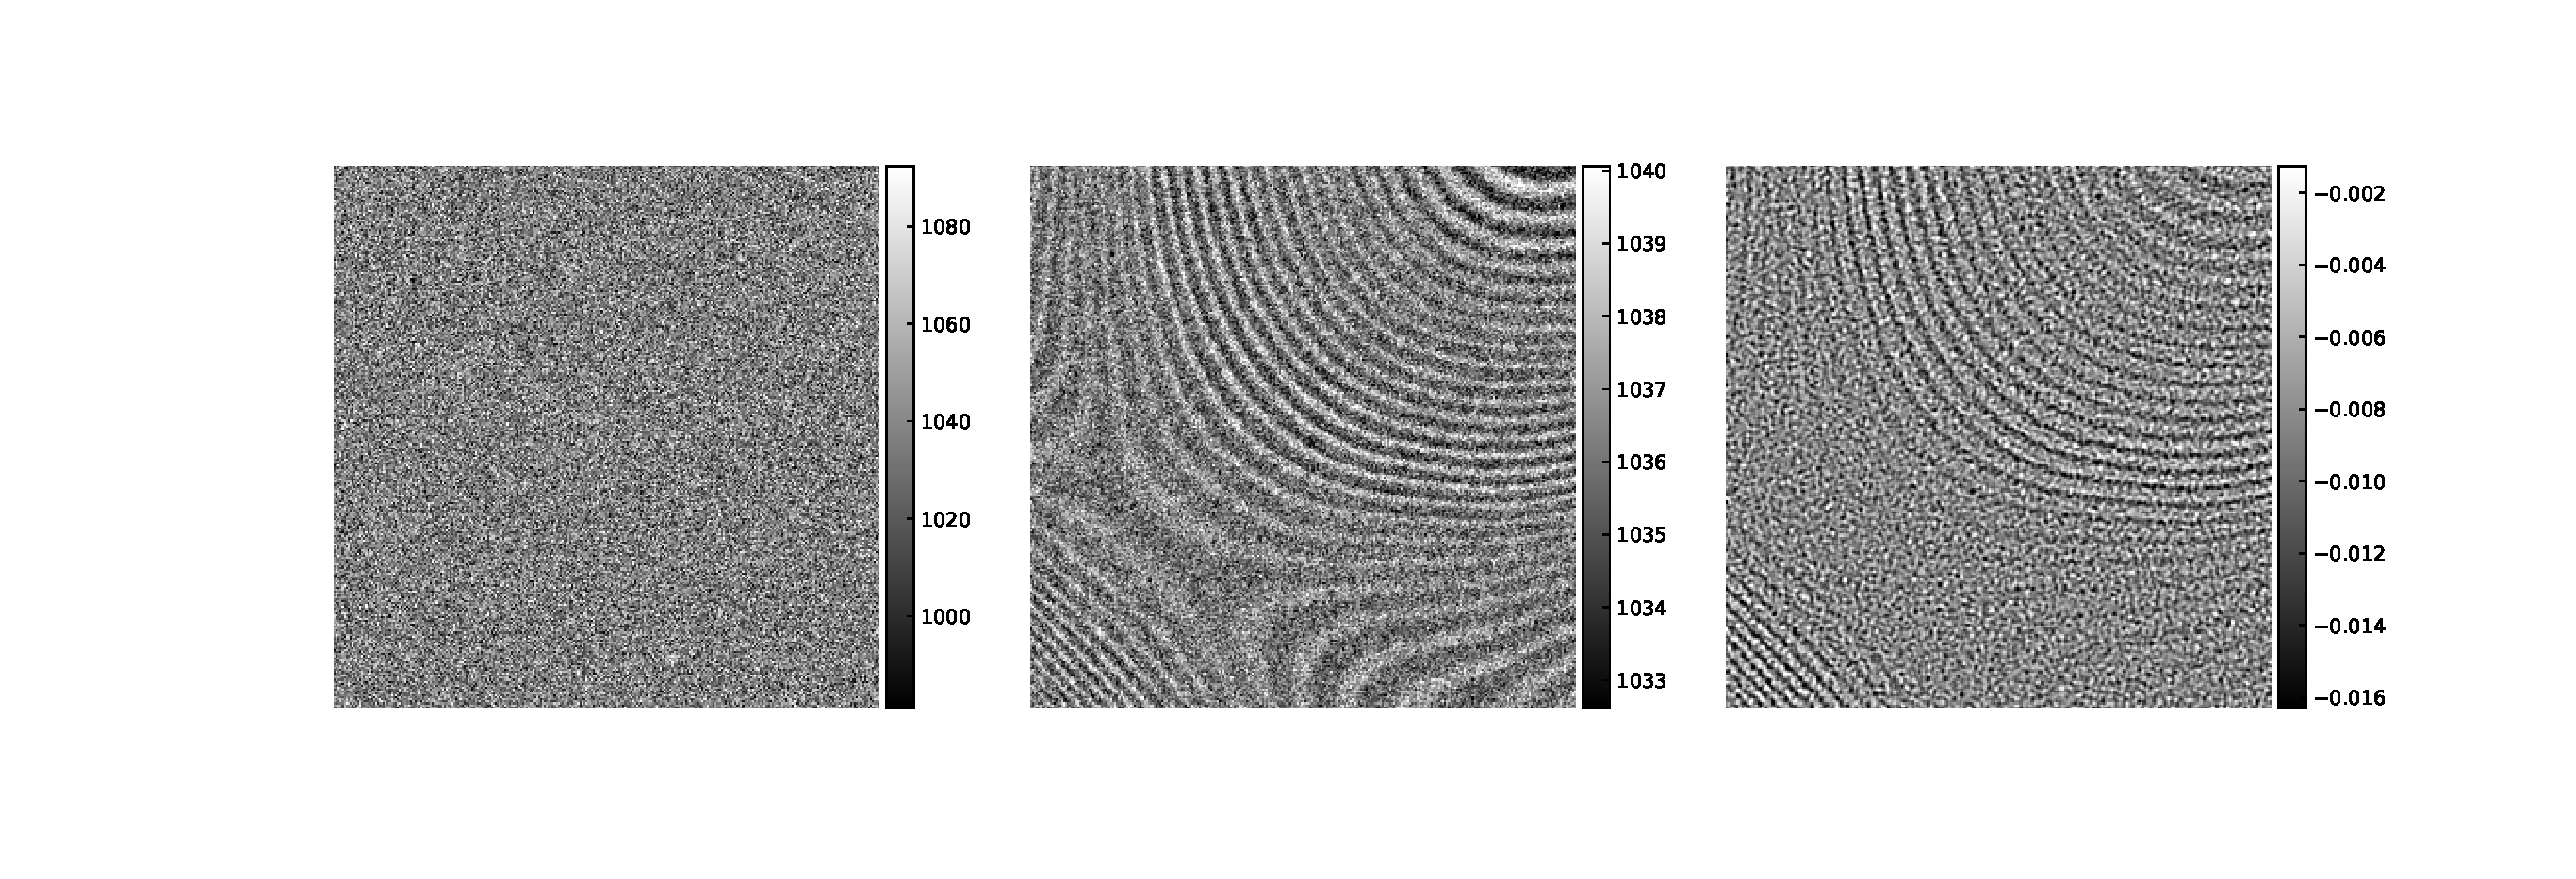
\includegraphics[scale = 0.4]{LSST-skybg-image.eps}
\caption{{\it Left panel:} Simulated LSST midnight sky background image. {\it Middle panel:} A Gaussian filter with kernel size of 16 by 16 pixel applied to the simulated image. {\it Right panel:} A Ricker hat filter of 60 by 60 pixel kernel size applied to the image. Color bar in the right and middle panel shows number of electrons per pixel. Color bar in left panel shows the residual of the image after applying the filter.}
\label{fig:lsst-image}
\end{figure*}
%%%%%%%%%%%%%%%%%%%%%

%%%%%%%%%%%%%%%%%%%%%
\begin{figure*}[tbh]
\centering
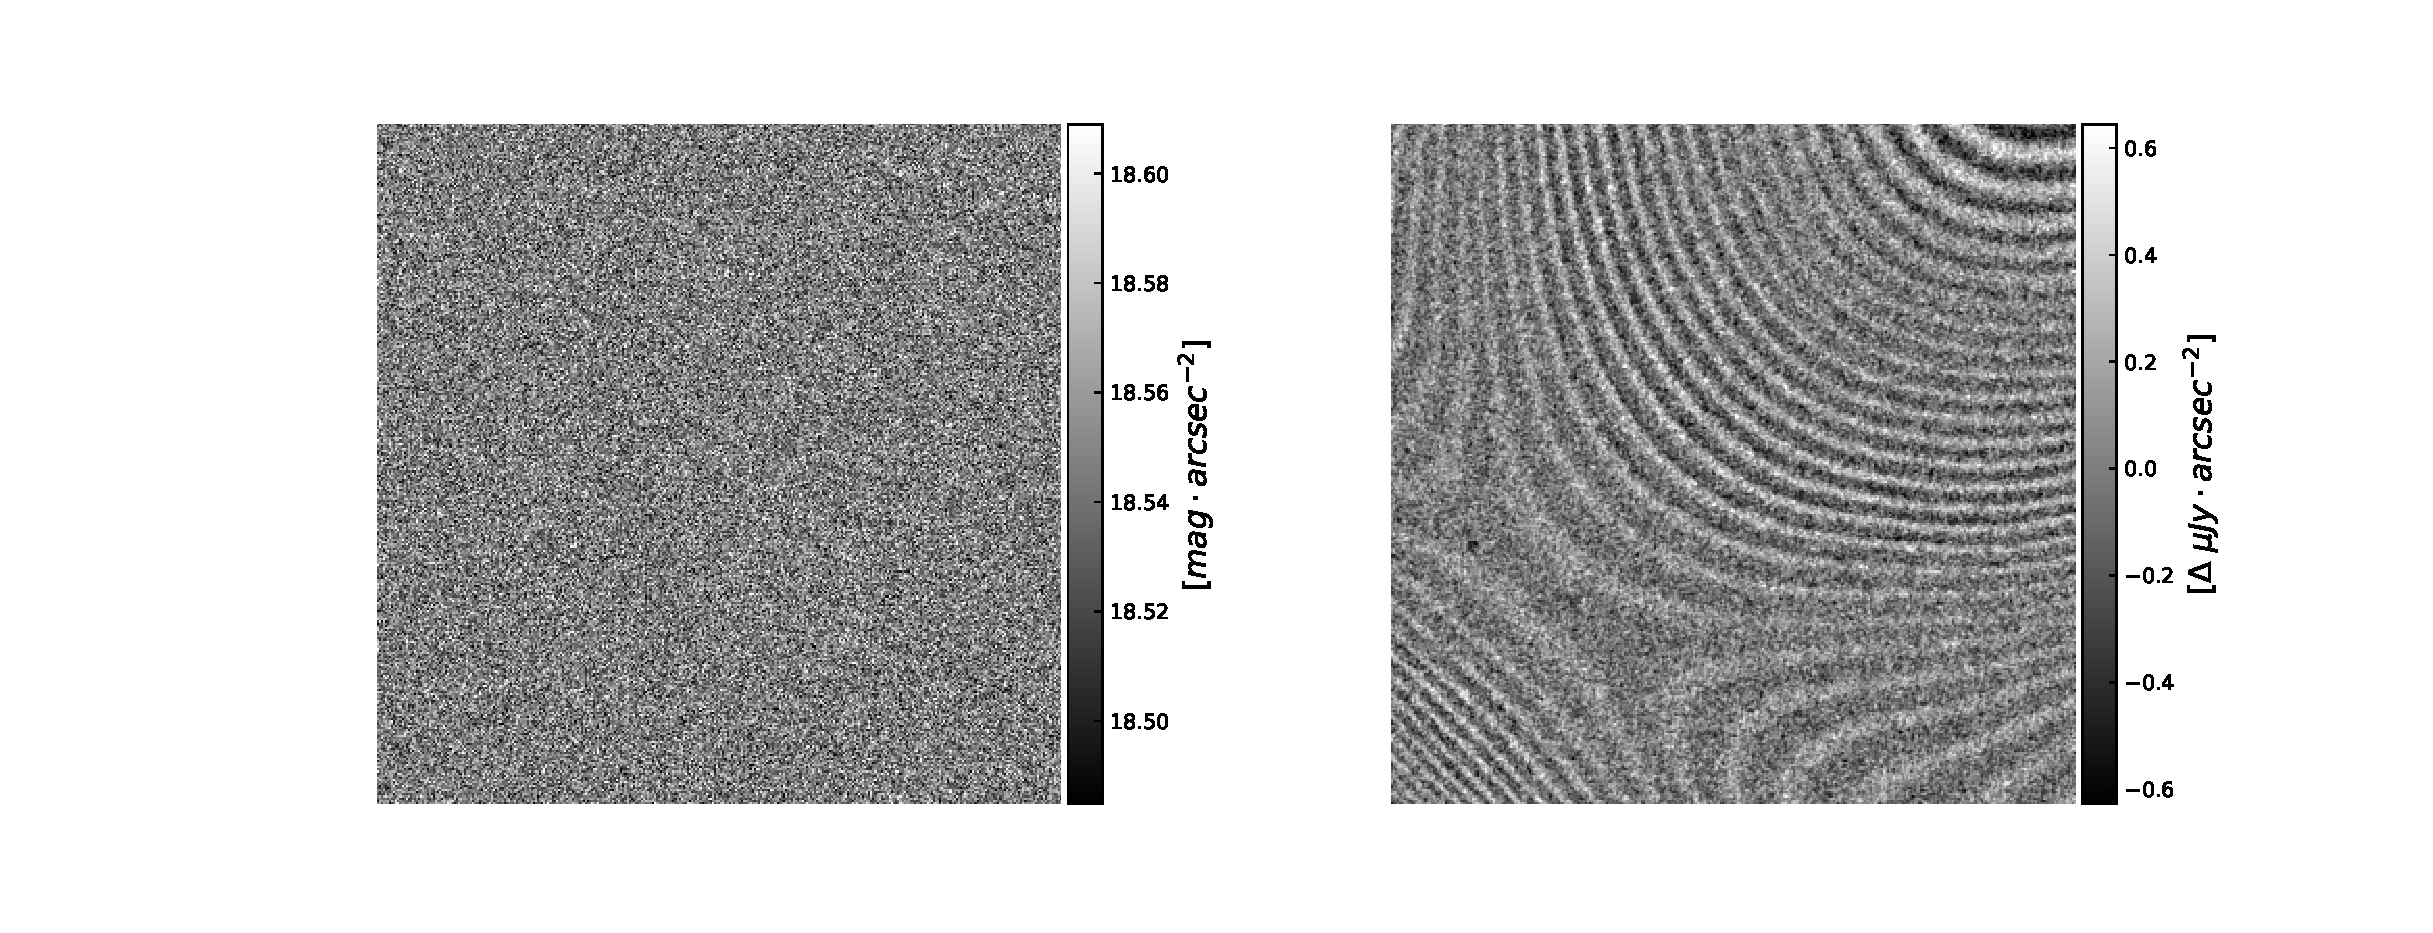
\includegraphics[scale = 0.45]{LSST-skybg-mag-image.eps}
\caption{{\it Left panel:} Simulated LSST midnight y filter sky background image. Colorbar shows the sky background brightness. {\it Righte panel:} A Gaussian filter with kernel size of 16 by 16 pixel applied to the simulated image.  Color bar shows the deviation ($\Delta \mu$) in brightness (millimag) from the mean value.}
\label{fig:lsst-image}
\end{figure*}
%%%%%%%%%%%%%%%%%%%%%

After validating the fringing model with MonoCam and HSC optics, we simulated the expected fringing pattern of e2v-CCD250-321 based on LSST setups as described in section~\ref{sec:LSST optic}.  In Figure~\ref{fig:LSST_sims}, we compared the simulated fringing patterns for two cases in terms of the CCD's location on the LSST focal plane, which only differ in their angle distribution of incident beam as shown in Figure~\ref{fig:batoid-angle-dist}. Compared with the values calculated in previous sections, the fringing amplitude for LSST decreased to $0.2\%$. This is caused by the fact that the wide range of incident angle of LSST optics decreases the overall fringing amplitude when incorporating the beams coming from all the angles in the simulation. As the sensor being placed far away from the center of field of view, the fringing amplitude decreases further to $0.04\%$. This is because the light arriving at the edge of the focal plane does not come from an exact $f/1.23$ beam due to the LSST optical design~\citep{Olivier08}, as manifested by the green and blue rays in Figure~\ref{fig:batoid-light-tracing}. This leads to a wider range of incident angle, which decreases the overall fringing amplitude when incorporating the beams coming from all the angles in the simulation. 

To check if fringing at this level should be considered in the LSST sky background subtraction in LSST data measurement pipeline, we applied two filters that are widely used in image processing for astronomy image, to the simulated LSST sky image in the case of the sensor being placed in the center of the focal plane. The first one is a Gaussian filter, which are commonly used to reduce noise level in the image, with kernel size of 16 by 16 pixel. The other is the Ricker wavelet filter (also known as the Mexican hat filter), which are used for image background subtraction, with kernel size of 60 by 60 pixel. The results are presented in Figure~\ref{fig:lsst-image}. As it is shown in the middle panel of Figure~\ref{fig:lsst-image}, the fringing pattern become prominent, with a coherent variation of a few electrons across the image, after applying the Gaussian filter. The variation of a few electrons over the image caused by the fringing pattern might still impact measurements of low surface brightness objects such as ultra diffuse galaxy. Similar patterns also appear in the residual image for implementation the Mexican hat filter as shown in the left panel in Figure~\ref{fig:lsst-image}. Thus, we conclude that despite of the low level of fringing inferred from simulation, the effect of fringes is still nontrivial in sky image. And a fringing removal algorithm is recommended should be included in the LSST Data Management pipeline.

%%%%%%%%%%%%%%%%%%%%%%%%%%%%%%%%%%%%%%%%%%%%%%

\section{Summary}
We have presented a fringing model for e2v-CDD250 sensors implemented on the LSST focal plane. We have verified that these observed fringes in e2v CCDs from SLAC-TS8 are caused by the thickness variations of the epoxy layer that glues the sensor and the support silicon together. We have shown that this model allows us to simulate the fringing patterns accurately observed in lab data on a pixel-by-pixel level. 

We have shown that with sufficient flat field data taken with close wavelength spacing ($< 10nm$) and under certain assumptions for the illumination setups, such as illumination bandwidth and incident angle, an underlying thickness map as a function of pixel position can be derived for each sensor via the fitting algorithm adopted from previous studies. Based on the derived thickness map, we have successfully reproduced the fringing patterns observed in nine e2v sensors in RTM-020 on LSST focal plane from SLAC-TS8. %We plan to implement the model to fit for all other e2v sensors used on LSST focal plane.

We have demonstrated that, by incorporating all the relevant factors rising from telescope optics and OH emission lines that dominates the night sky spectra into the fringing model, we are able to recover the observed fringing amplitude for MonoCam \citep{Brooks17} and HSC. We then use this model to predict the fringing pattern in LSST real sky images and find that the simulated LSST fringing amplitude ranges from $0.04\%$  to $0.2\%$ depending the location of a CCD on the focal plane. Finally, we verify that fringes will become nontrivial during image processing and reduction process for LSST. Table \ref{tbl:fringing summary} summaries all the simulation results in terms of different optics setups and conditions. This fringing simulation model can be readily implemented into the LSST-DESC image simulation tool (imSim).

\begin{deluxetable*}{ccccccc}[hbt] \label{tbl:fringing summary}
\tablecaption{Simulated fringing amplitude of e2v sensor for different optic setup}
\tablenum{2}
\tablecolumns{7}
\tablehead{
\colhead{} &
\colhead{Optics} &
\colhead{Temperature} &
\colhead{Source of fringing} &
\colhead{Simulation setup} &
\colhead{Observed amplitude} &
\colhead{Simulated amplitude}
}
\startdata
 SLAC-TS8 & $f/\infty$ & $-90\degree C$ & Epoxy & Monochromator ($960nm$) &$\sim 2\%$ & $2\%$   \\
 MonoCam & $f/4$ & $-120\degree C$ & Epoxy &OH lines $+$ LSST y band & $\sim 2\%$ &  $1.5\%$\\
 HSC & $f/2$ & $-100\degree C$ & Silicon($\sim 200\mu m$) &OH lines $+$ HSC y band &$0.2\%\sim 0.6\%$ & $0.3\%$\\
 LSST & $f/1.23$ & $-100\degree C$ &Epoxy & OH lines $+$ LSST y band & $ -$ & $ 0.04\%\sim 0.2\%$ \\
\enddata

\end{deluxetable*}

\acknowledgements
\textbf{We are grateful to Pierre Antiogus, Jim Chiang, Mike Jarivs, Lee Kelvin, David Kirkby, Josh Meyers, Rorbert Lupton, Andrei Nomerotski, Paul O'Connor, Andy Rasmussen, Aaron Roodman and Peter Yoachim for helpful discussions.}
LSST is a public-private partnership. Funding for design and development activity comes from the National Science Foundation, private donations, grants to universities, and in-kind support at Department of Energy laboratories and other LSSTC Institutional Members. This research is supported by the U.S. Department of Energy, Office  of  Science,  Office  of  High  Energy  Physics  under Award Number **-**-*******.

\newpage
\bibliography{reference}{}
\bibliographystyle{aasjournal}


%\appendix
%%%%%% Plot: e2v-CCD-321 MAP and Simulated Results
%\begin{figure*}[h]
%\centering
%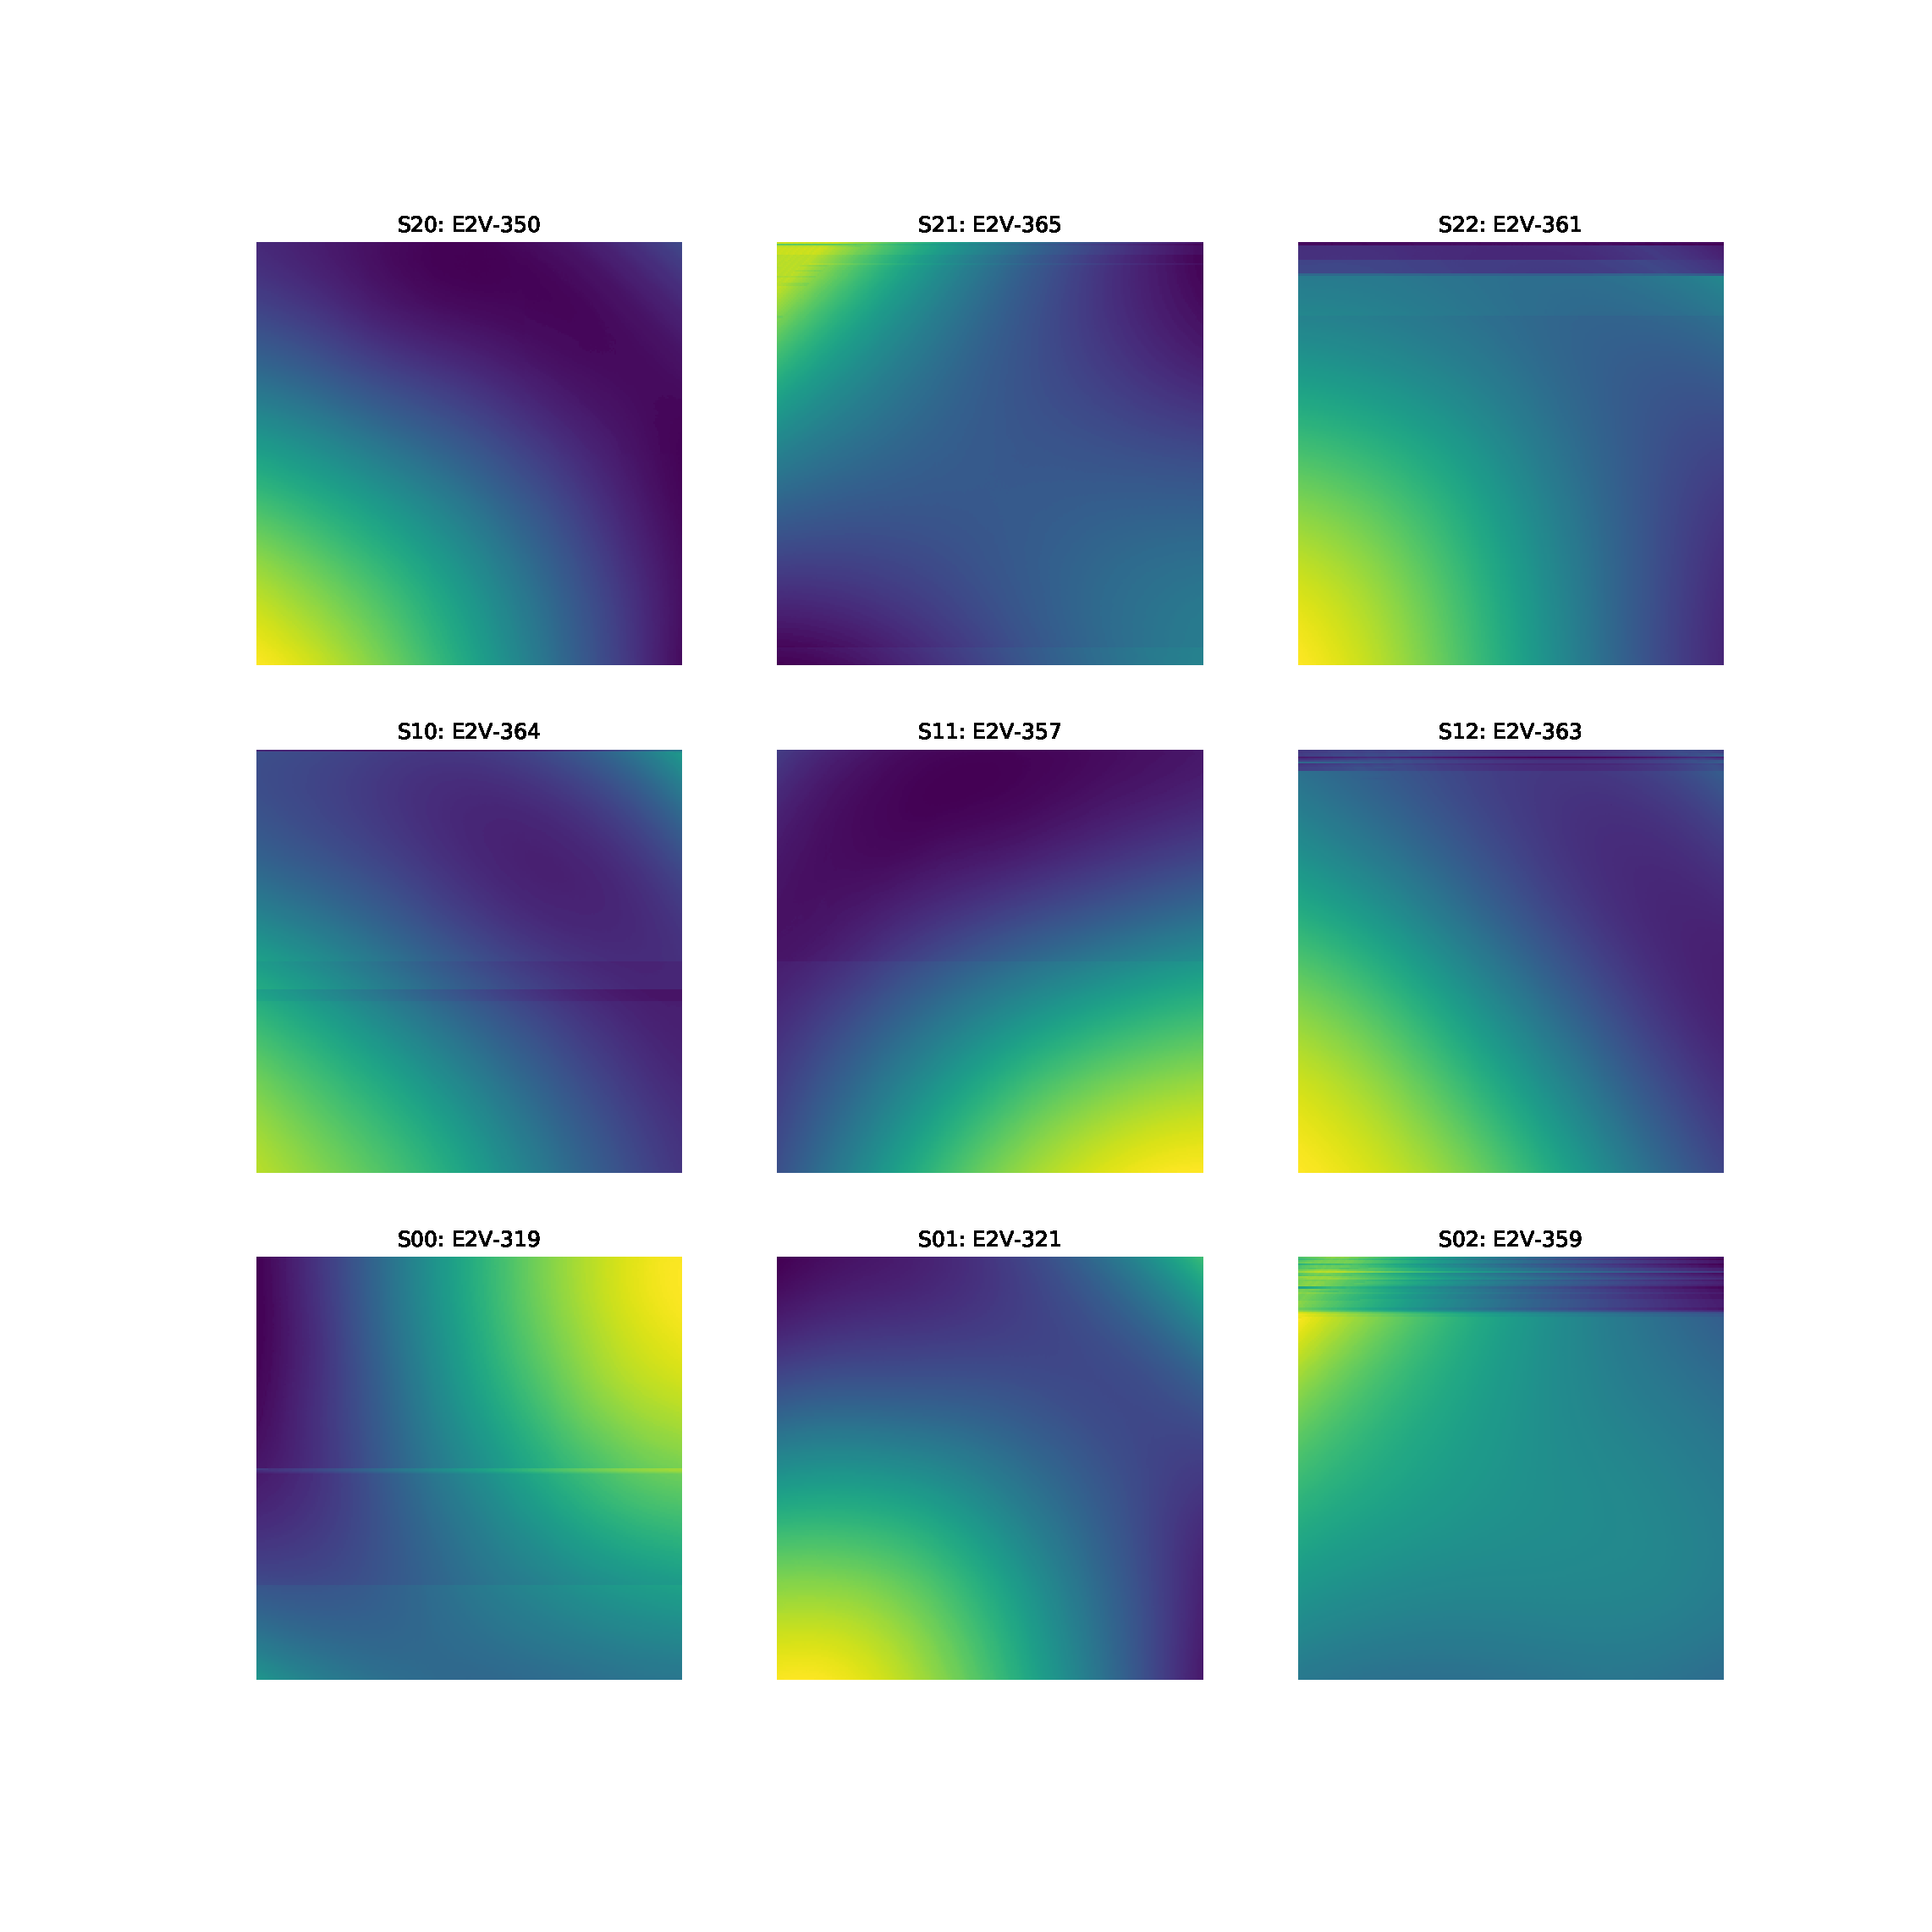
\includegraphics[scale = 0.45]{RTM-020-Maps.eps}
%\caption{Simulated fringing pattern based on derived epoxy thickness map for nine e2v CCDs in RTM-020}
%\label{fig:RTM-020-MAPS}
%\end{figure*}

%\begin{figure*}[h]
%\centering
%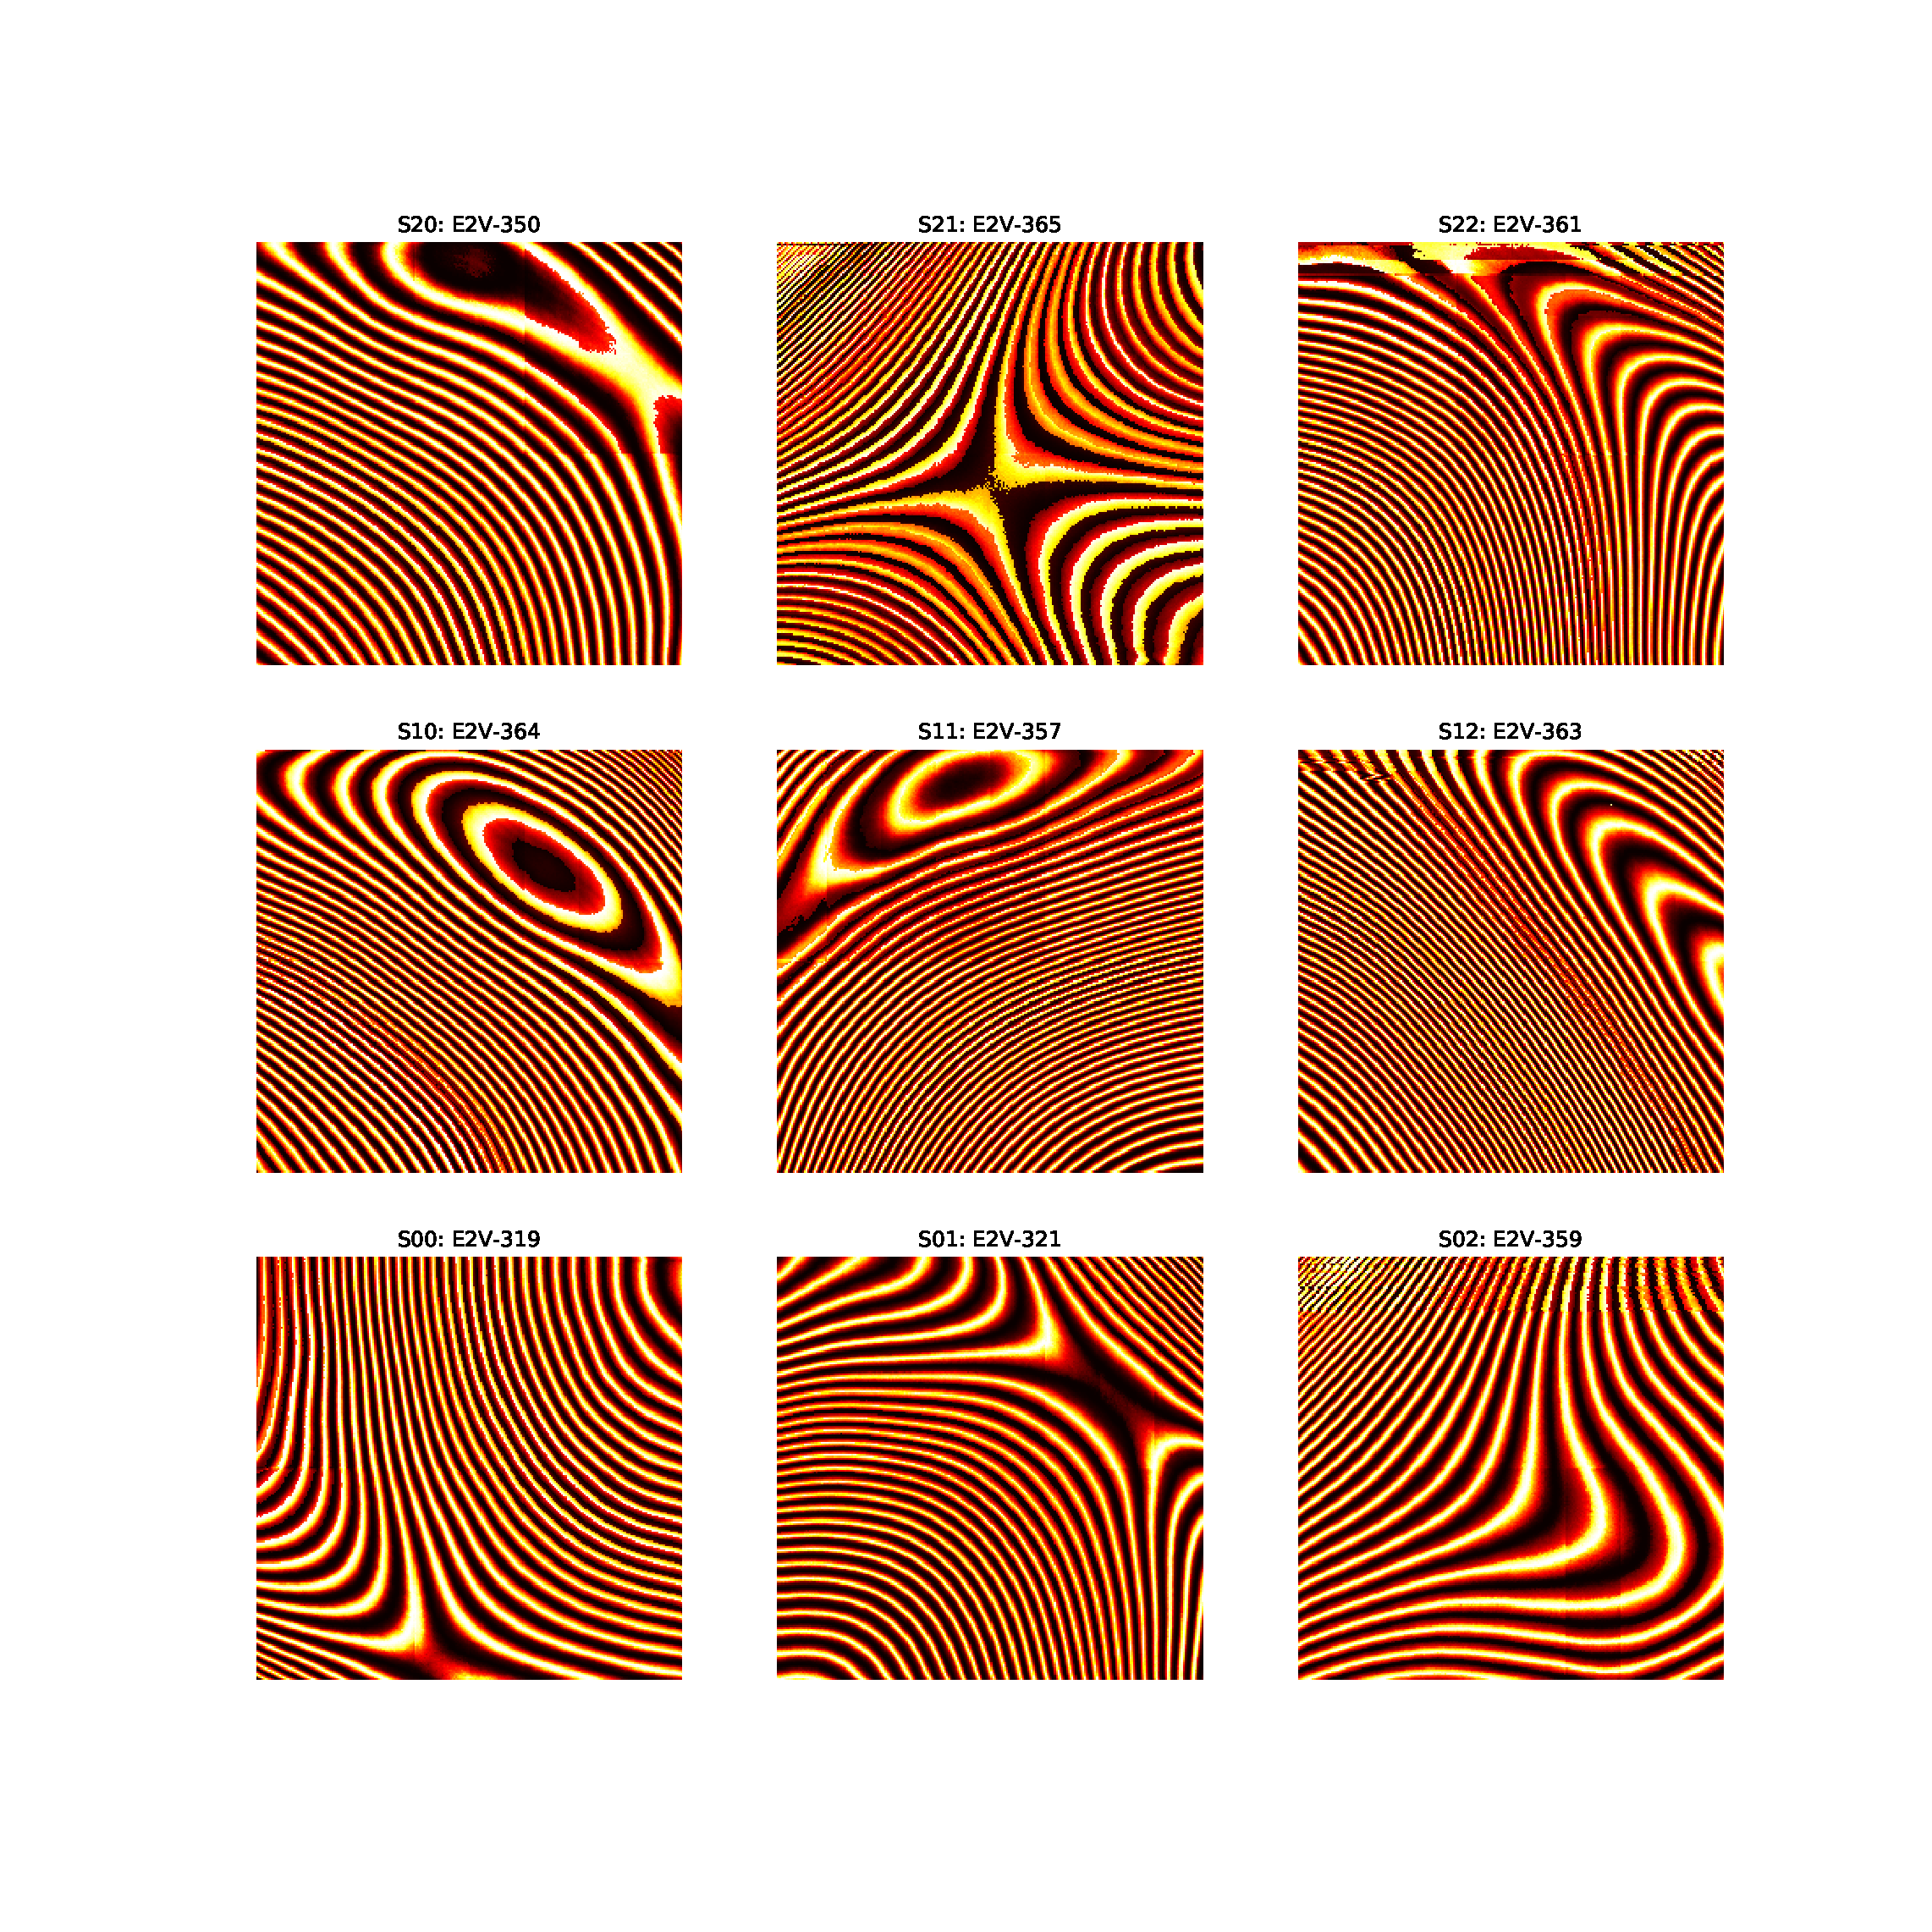
\includegraphics[scale = 0.45]{RTM-020-Sim.eps}
%\caption{Simulated fringing pattern (with illumination bandwidth being a delta function at 960nm) based on derived epoxy thickness map for nine e2v CCDs in RTM-020}
%\label{fig:RTM-020-SIMS}
%\end{figure*}

%%%%%%%
\end{CJK*}
\end{document}
